\documentclass[a4paper, 12pt]{article}
\usepackage[a4paper,top=1.5cm, bottom=1.5cm, left=1cm, right=1cm]{geometry}

% Работа с русским языком
\usepackage[utf8]{inputenc}
\usepackage{mathtext}                % русские буквы в формулах
\usepackage[english, russian]{babel} % локализация и переносы

\usepackage{booktabs}
\usepackage{graphicx}   % Вставка изображений
\usepackage{float}      % "Плавающие" изображения3
\usepackage{wrapfig}    % Обтекание фигур (таблиц, картинок и прочего)
\usepackage{subfig}
\graphicspath{ {./images/} }

\usepackage{tabularx}
\usepackage{multirow}
\usepackage{amsmath}
\usepackage{amsfonts}
\usepackage{indentfirst}
\usepackage{longtable}
\graphicspath{{pictures/}}
\usepackage{natbib}
\usepackage{bm}

%%% Колонтитулы
\usepackage{titleps}
\newpagestyle{main}{
	\setheadrule{0.4pt}
	\sethead{Скин-эффект в полом цилиндре}{}{}
	\setfootrule{0.4pt}                       
	\setfoot{ФРКТ МФТИ, 2023}{}{\thepage} 
}
\pagestyle{main}  

\begin{document}
    \begin{titlepage}
	\begin{center}
            {\large МОСКОВСКИЙ ФИЗИКО-ТЕХНИЧЕСКИЙ ИНСТИТУТ (НАЦИОНАЛЬНЫЙ ИССЛЕДОВАТЕЛЬСКИЙ УНИВЕРСИТЕТ)}
	\end{center}
 
	\begin{center}
		{\large Физтех-школа радиотехники и компьютерных технологий}
	\end{center}
	
	\vspace{8cm}
	{\LARGE
		\begin{center}
                {\bf Отчёт о выполнении лабораторной работы 3.7.1}\\
                Скин-эффект в полом цилиндре
		\end{center}
	}
	\vspace{5cm}
	\begin{flushright}
		{\Large Автор:\\ Тихонов Дмитрий Романович, \\
			\vspace{0.2cm}
			студент группы Б01-206}
	\end{flushright}
	\vspace{5cm}
	\begin{center}
		\Large Долгопрудный, 2023
	\end{center}
    \end{titlepage}


    \section{Введение}

    \noindent \textbf{Цель работы:} исследовать явление проникновения переменного магнитного поля в медный полый цилиндр. \\

    \noindent \textbf{В работе используются:} : генератор сигналов АКИП–3420, соленоид, намотанный на полый цилиндрический каркас, медный экран в виде полого цилиндра, измерительная катушка, амперметр, вольтметр, двухканальный осциллограф GOS–620, RLC-метр.
    
    \section{Теоретические сведения}
    
    \subsection{Скин-эффект для полупространства}

    \begin{wrapfigure}{l}{6 cm}
        \centering
        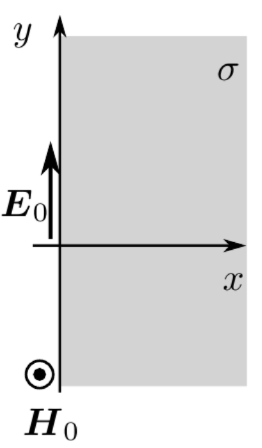
\includegraphics[width=0.2\textwidth]{images/flat_se.png}
        \caption{Скин-эффект в плоской геометрии}
        \label{fig:flat_se}
    \end{wrapfigure}

    Рассмотрим квазистационарное поле внутри проводящей среды в простейшем плоском случае. Пусть вектор $\bm{E}$ направлен всюду вдоль оси $y$ (рис.\ref{fig:flat_se}) и зависит только от координаты $x$, т. е. ${E_x} = {E_z} \equiv 0$, $E_y \equiv E_y(x,t)$. Пренебрегая \textit{током смещения} в уравнениях поля, запишем
    
    \begin{equation}
        \operatorname{rot} \bm{H} = \sigma \bm{E}.
        \label{eq:stationary_1}
    \end{equation}
    
    Возьмём ротор обеих частей (\ref{eq:stationary_1}), считая проводимость $\sigma$ постоянной:
    
    \begin{equation}
        \operatorname{rot} \operatorname{rot} \bm{H} = \operatorname{grad} \operatorname{div} \bm{H} - \nabla^2 \bm{H} = - \nabla^2 \bm{H} = \sigma \operatorname{rot} \bm{E}
    \end{equation}

    Подставим закон электромагнитной индукции ($\operatorname{rot} \bm{E} = - \frac{\partial \bm{B}}{\partial t}$) и \textit{материальное уравнение} для векторов магнитного поля ($\bm{B} = \mu \mu_0 \bm{H}$): 
    
    \begin{equation}
        \nabla^2 \bm{H} = \sigma\mu\mu_0\frac{\partial\bm{H}}{\partial t} 
        \label{eq:stationary_H}
    \end{equation}

    Точно такое же уравнение имеет место и для $\bm{E}$:

    \begin{equation}
        \nabla^2 \bm{E} = \sigma\mu\mu_0\frac{\partial\bm{E}}{\partial t} 
        \label{eq:stationary_E}
    \end{equation}

    Подставляем в (\ref{eq:stationary_E}) соотношение для электрического поля $E_y = E_y(x,t)$:
    
    \begin{equation}
        \frac{\partial^2 E_y}{\partial x^2} = \sigma\mu\mu_0\frac{\partial E_y}{\partial t}
        \label{eq:stationary_E_y}
    \end{equation}
    
    Пусть полупространство $x > 0$ заполнено проводящей средой с проводимостью $\sigma$, а на границе $x = 0$ задано электрическое поле, изменяющееся по гармоническому закону: $E_y = E_0 e^{i \omega t}$. Будем искать решение уравнения (\ref{eq:stationary_E_y}) также в виде гармонической функции:

    \begin{equation*}
        E_y(x,t) = E(x) e^{i \omega t},
    \end{equation*}

    где $E(x)$ -- комплексная амплитуда колебаний поля, зависящая от координаты $x$. После подстановки в (\ref{eq:stationary_E_y}) получим уравнение на функцию $E(x)$:

    \begin{equation}
        \frac{d^2 E}{dx^2} = i\omega\sigma\mu\mu_0 E.
        \label{eq:stationary_diffur}
    \end{equation}

    Решение будеим искать в виде

    \begin{equation}
        E(x) = E_0 e^{\alpha x},
        \label{eq:stationary_solve}
    \end{equation}

    где $\alpha$ -- комплексная константа. Подставляя (\ref{eq:stationary_solve}) в (\ref{eq:stationary_diffur}), получим, что

    \begin{equation}
        \alpha = \pm \frac{1+i}{\sqrt{2}} \sqrt{\omega\sigma\mu\mu_0}.
    \end{equation}

    Для полубесконечной среды физический смысл имеет только решение со знаком <<$-$>>, соответствующее стремлению к нулю амплитуды поля. Окончательное решение уравнения (\ref{eq:stationary_E_y}) для нашего случая:

    \begin{equation}
        E_y(x,t) = E_0 e^{-x/\delta} e^{i(\omega t - x/\delta)},
    \end{equation}

    где

    \begin{equation}
        \delta = \sqrt{\frac{2}{\omega\sigma\mu\mu_0}}.
        \label{eq:delta}
    \end{equation}

    Расстоянием $\delta$, на котором амплитуда поля уменьшается в $e$ раз, называют \textit{глубиной проникновения} поля или \textit{скиновой} длиной. С ростом частоты $\omega$ электрическое поле всё более <<вытесняется>> к поверхности проводника. Это явление называется \textit{скин-эффектом}.

    \subsection{Скин-эффект в полом цилиндре}

    \begin{wrapfigure}{l}{0.3\textwidth}
        \centering
        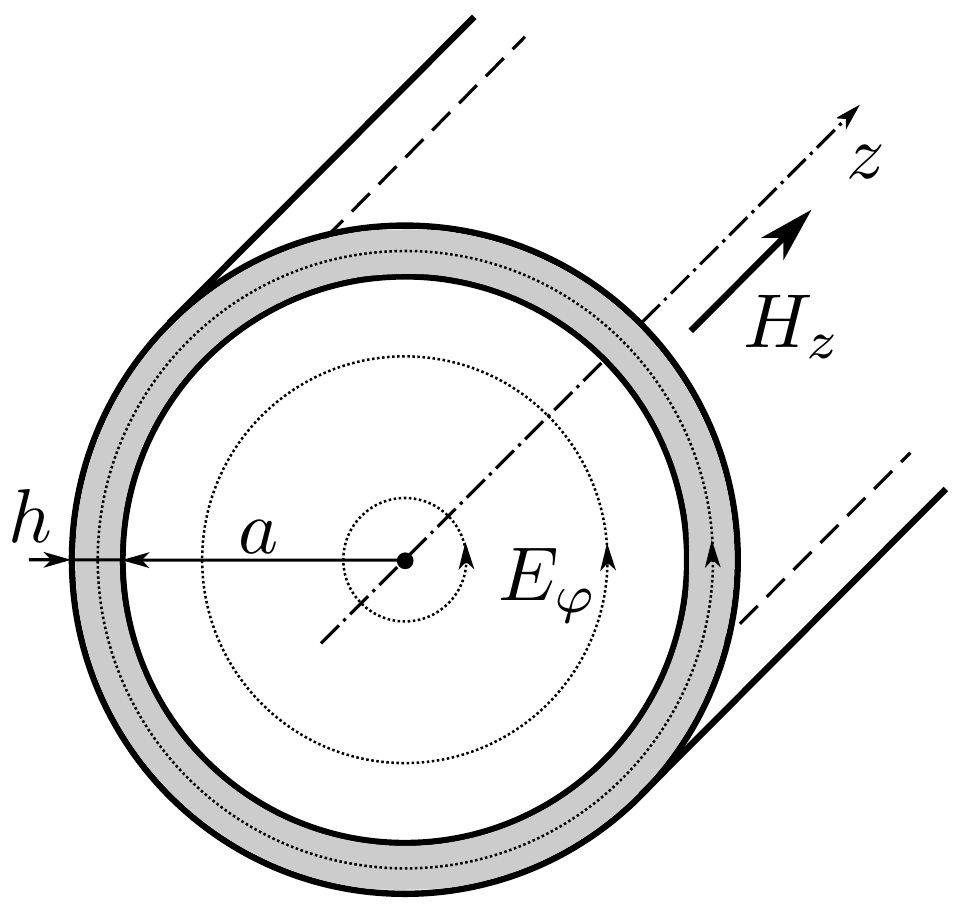
\includegraphics[width=0.25\textwidth]{images/cyl_se.png}
        \caption{Электрическое и магнитное поле в тонкостенном цилиндре}
        \label{fig:cyl_se}

        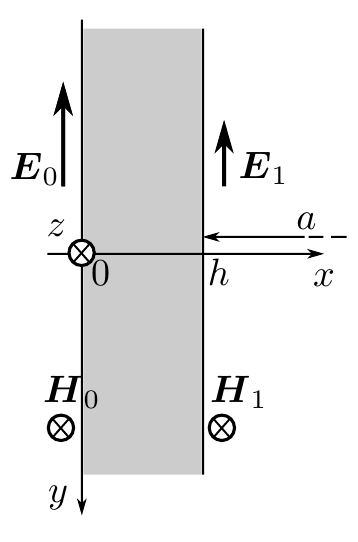
\includegraphics[width=0.25\textwidth]{images/cyl_flat_se.png}
        \caption{Поле в стенке цилиндра}
        \label{fig:cyl_flat_se}
        
    \end{wrapfigure}

    Пусть цилиндр достаточно длинный, так что в нём можно пренебречь краевыми эффектами. В этом приближении магнитное поле $\bm{H}$ всюду направлено по оси системы (ось $z$), а вихревое электрическое поле $\bm{E}$ будет всюду перпендикулярно радиусу (рис. \ref{fig:cyl_se}). Для ненулевых компонент поля можно записать

    \begin{equation*}
        H_z = H(r) e^{i \omega t}, \hspace{4 mm} E_\varphi = E(r) e^{i \omega t},
    \end{equation*}

    где $H(r)$ и $E(r)$ -- комплексные амплитуды колебаний соответствующих полей, зависящие только от расстояния $r$ до оси системы. Заметим, что на границе цилиндра должны быть непрерывны касательные к поверхности компоненты как $\bm{E}$, так и $\bm{B}$, поэтому функции $E(r)$ и $H(r)$ непрерывны во всей исследуемой области.

    Поскольку внутри цилиндра ток отсутствует, магнитное поле там является однородным: $H_z(r,t) = H_1 e^{i \omega t}$, где $H_1 = \operatorname{const}$ -- амплитуда поля на внутренней поверхности цилиндра. По теореме об электромагнитной индукции:

    \begin{equation*}
        E_\varphi \cdot 2\pi r = -\mu_0 \pi r^2 \cdot \frac{d H_z}{dt} \hspace{4 mm} \rightarrow \hspace{4 mm} E(r) = -\frac{1}{2} \mu_0 r \cdot i \omega H_1. 
    \end{equation*}

    Отсюда, получим связь амплитуд колебаний электрического и магнитного полей на внутренней ($r = a$) границе цилиндра:

    \begin{equation}
        E_1 = -\frac{1}{2} i \omega a \mu_0 H_1.
    \end{equation}

    Поле внутри тонкой стенки цилиндра описывается уравнением скин-эффекта (\ref{eq:stationary_E_y}) в плоской геометрии (рис. \ref{fig:cyl_flat_se}). Тогда надо решить уравнение (\ref{eq:stationary_H}) с граничными условиями. Решая уравнение, получим связь между $H_0$ и $H_1$:

    \begin{equation}
        H_1 = \frac{H_0}{\ch{\alpha h} + \frac{1}{2} \alpha a \sh{(\alpha h)}},
        \label{eq:flat_cyl}
    \end{equation}

    где

    \begin{equation}
        \alpha = \sqrt{i \omega\sigma\mu_0} = \frac{1 + i}{\delta} = \frac{\sqrt{2}}{\delta} e^{i \pi/4}.
        \label{eq:alpha_flat_cyl}
    \end{equation}

    Рассмотрим предельные случаи (\ref{eq:flat_cyl}).

    \begin{enumerate}
        \item При \textit{малых частотах} толщина скин-слоя превосходит толщину цилиндра $\delta \gg h$. Тогда $\lvert \alpha h \rvert \ll 1$, поэтому $\ch \alpha h \approx 1$, $\sh \alpha h \approx \alpha h$ и

        \begin{equation}
            H_1 \approx \frac{H_0}{1 + i \frac{ah}{\delta^2}}.
            \label{eq:nu_ll_1}
        \end{equation}

        Отношение модулей амплитуд здесь будет равно 

        \begin{equation}
            \frac{\lvert H_1 \rvert}{\lvert H_0 \rvert} = \frac{1}{\sqrt{1 + \left(\frac{ah}{\delta^2}\right)^2}} = \frac{1}{\sqrt{1 + \frac{1}{4} \left( ah\sigma\mu_0 \omega \right)^2}}.
            \label{eq:nu_ll_2}
        \end{equation}

        При этом колебания $H_1$ отстают по фазе от $H_0$ на угол $\psi$, определяемый равенством 

        \begin{equation}
            \tg \psi = \frac{ah}{\delta^2}.
            \label{eq:tg_psi}
        \end{equation}

        \item При достаточно \textit{больших частотах} толщина скин-слоя станет меньше толщины стенки: $\delta \ll h$. Тогда $\lvert \alpha h \rvert \gg 1$ и $\lvert \alpha a \rvert \gg 1$, а также $\sh (\alpha h) \approx \ch (\alpha h) \approx \frac{1}{2} e^{\alpha h}$. Выражение (\ref{eq:flat_cyl}) с учётом (\ref{eq:alpha_flat_cyl}) переходит в

        \begin{equation}
            \frac{H_1}{H_0} = \frac{4}{\alpha a} e^{-\alpha h} = \frac{2 \sqrt{2} \delta}{a} e^{-\frac{h}{\delta}} e^{-i\left( \frac{\pi}{4} + \frac{h}{\delta} \right)}.
        \end{equation}

        При этом поле внутри цилиндра запаздывает по фазе на 

        \begin{equation}
            \psi = \frac{\pi}{4} + \frac{h}{\delta} = \frac{\pi}{4} + h\sqrt{\frac{\omega \sigma \mu_0}{2}}.
            \label{eq:psi}
        \end{equation}
        
    \end{enumerate}

    

    \section{Методика измерений и используемое оборудование}

    \subsection{Экспериментальная установка}

    Схема экспериментальной установки для исследования скин–эффекта в полом цилиндре изображена на рис. \ref{fig:installation_1}.

    \begin{figure}[H]
        \centering
        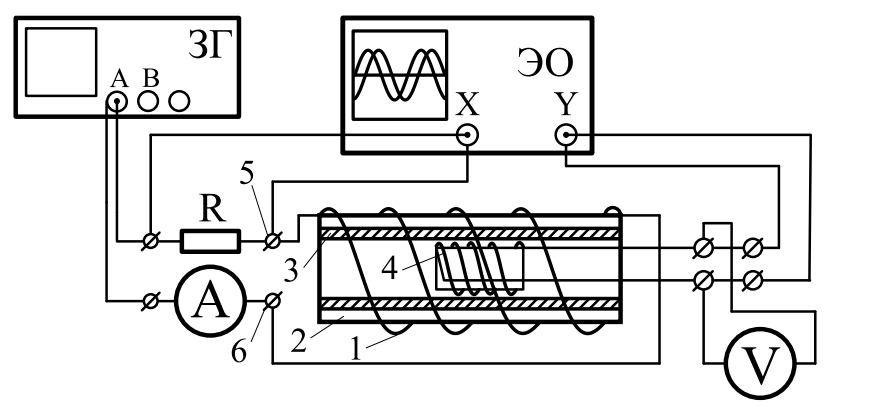
\includegraphics[width = 14 cm]{images/installation_1.png}
        \caption{Экспериментальная установка для изучения скин-эффекта}
        \label{fig:installation_1}
    \end{figure}

    Переменное магнитное поле создается с помощью соленоида 1, намотанного на цилиндрический каркас 2 из поливинилхлорида, который подключается к генератору сигналов (ЗГ) АКИП–3420 (канал А). Внутри каркаса расположен медный экран 3 в виде полого цилиндра. 
    
    \textit{Действующее} значение переменного тока в цепи соленоида измеряется цифровым амперметром <<А>>. \textit{Действующее} значение переменного напряжения на измерительной катушке 4 измеряется цифровым вольтметром <<V>>. В качестве амперметра и вольтметра используются два мультиметра GDM–8245.
    
    Для измерения сдвига фаз между током в цепи соленоида и напряжением на измерительной катушке используется двухканальный осциллограф GOS–620 (ЭО).

    Схема экспериментальной установки для нахождения проводимости $\sigma$ по изменению индуктивности катушки $L$ изображена на рис. \ref{fig:installation_2}. \textit{RLC}-метр, измеряющий индуктивность, подключается к катушке 1 через клеммы 5 и 6 на панеле установки. Другие приборы при этом должны быть отсоединены от цепи, т.к. \textit{RLC}-метр измеряет индуктивность активным образом.

    \begin{figure}[H]
        \centering
        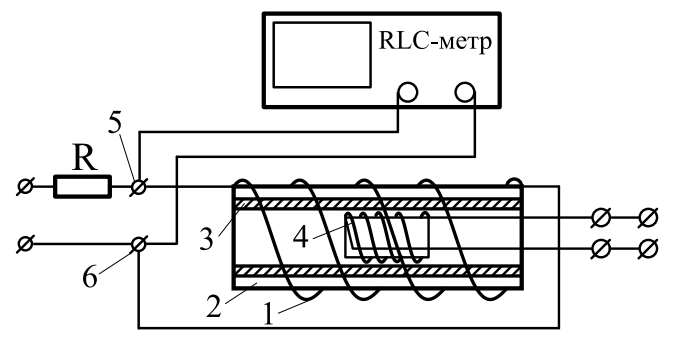
\includegraphics[width = 14 cm]{images/installation_2.png}
        \caption{Экспериментальная установка для изучения скин-эффекта}
        \label{fig:installation_2}
    \end{figure}

    \subsection{Измерение отношения амплитуд магнитного поля внутри и вне экрана}

    С помощью вольтметра $V$ измеряется действующее значение ЭДС индукции, которая возникает в измерительной катушке, находящейся в переменном магнитном поле $H_1 e^{i\omega t}$:

    \begin{equation*}
        U(t) \propto \frac{dB_1(t)}{dt} = -i \omega H_1 e^{i \omega t}.
    \end{equation*}

    Поле вне экрана $\lvert H_0 \rvert$ пропорционально току $I$ в цепи соленоида, измеряемому амперметром $A$:

    \begin{equation*}
        \lvert H_0 \rvert \propto I.
    \end{equation*}

    Отсюда, 

    \begin{equation}
        \frac{\lvert H_1 \rvert}{\lvert H_0 \rvert} = \operatorname{const} \cdot \frac{U}{\nu I} = \frac{\xi}{\xi_0},
    \end{equation}

    где константу $\xi_0$ можно определить из условия $\lvert H_1 \rvert/\lvert H_0 \rvert \rightarrow 1$ при $\nu \rightarrow 0$.

    \subsection{Определение проводимости материала экрана по фазовому сдвигу}

    Из формул (\ref{eq:tg_psi}) и (\ref{eq:delta}) следует линейная зависимость $\tg\psi$ от $\nu$, причем аппроксимирующая прямая должна проходить через начало координат.
    
    Как видно из выражения (\ref{eq:psi}), в области больших частот $\nu \gg 1/(\pi h^2 \sigma \mu_0)$ зависимость $\psi(\sqrt{\nu}) - \pi/4$ аппроксимируется прямой, проходящей через начало координат. По наклону этих прямых можно вычислить проводимость материала экрана.

    Заметим, что на схеме, изображённой на рис. \ref{fig:installation_1}, на входной канал $Y$ осциллографа подаётся сигнал с измерительной катушки, который пропорционален не полю внутри экрана, а его производной по времени, а это означает, что появляется дополнительный сдвиг по фазе на $\pi/2$. Поэтому измеренный по экрану осциллографа сдвиг по фазе между двумя синусоидами будет на $\pi/2$ больше фазового сдвига между магнитными полями вне и внутри экрана:

    \begin{equation}
        \varphi = \psi + \frac{\pi}{2}.
    \end{equation}

    \subsection{Влияние скин-эффекта на индуктивность катушки}

    Из-за скин эффекта индуктивность соленоида с медным цилиндрическим экраном внутри будет зависеть от частоты тока. Рассмотрим магнитный поток через катушку как сумму двух магнитных потоков: 1) пронизывающий область между катушкой и цилиндрическим экраном $\Phi_{out}$; 2) пронизывающий область за экраном $\Phi_{in}$:

    \begin{equation}
        \Phi = \Phi_{out} + \Phi_{in} = H_0 S_0 + H_1 S_1 = LI,
    \end{equation}

    где $H_0$, $H_1$ -- \textit{мгновенные} значения магнитного поля внутри и снаружи цилиндра при данном токе $I$; $S_0$, $S_1$ -- площади внешней и внутренней областей соответственно.

    Минимальная индуктивность будет, когда $\Phi_{in} = 0$, при этом:

    \begin{equation}
        L_{min} = \frac{\Phi_{out}}{I}.
    \end{equation}

    Выразим поток магнитного поля сквозь внутреннюю область $\Phi_{in}$ через поток сквозь внешнюю $\Phi_{out}$ при произвольном переменном токе $I$:

    \begin{equation}
        \Phi_{in} = H_1 S_1 = \frac{H_1 S_1}{H_0 S_0} \Phi_{out}.
    \end{equation}

    Максимальная индуктивность катушки достигается при максимальном потоке поля во внутренней области:

    \begin{equation}
        \Phi_{max} = \Phi_{out} + \Phi_{in}^{max} = H_0 (S_1 + S_0) = L_{max} I.
    \end{equation}

    Отсюда, 

    \begin{equation}
        \frac{S_1}{S_0} = \frac{L_{max} - L_{min}}{L_{min}} \Rightarrow L = L_{min} + \frac{L_{max} - L_{min}}{H_0/H_1}
    \end{equation}

    Используя формулы (\ref{eq:delta}) и (\ref{eq:nu_ll_1}), окончательно получаем зависимость индуктивности катушки от частоты:

    \begin{equation}
        \frac{L_{max} - L}{L - L_{min}} = (\pi ah\mu_0\sigma\nu)^2.
    \end{equation}

    Данная зависимость может быть аппроксимирована прямой, по углу наклона которой можно найти проводимость материала экрана $\sigma$.

    
    \section{Результаты измерений и обработка данных}

    Параметры нашей установки $d = 45$ мм, $h=1,5$ мм. Проводимость порядка $\sigma \sim 5\cdot 10^7$ См/м. Получаем оценку для частоты, при которой глубина проникновения равна толщине стенок цилиндра $\nu_h = 2250$ Гц.

    \subsection{Измерение проводимости через отношение амплитуд}

    В области низких частот (от $\sim 0,01 \nu_h$ до $0,05 \nu_h$) получили зависимость отношения $\xi = U/\nu I$ от частоты $\nu$. Результаты измерений представлены в таблице \ref{table:amplitude}.

    \begin{table}[H]
        \centering
        \begin{tabular}{|c|c|c|c|c|}
        \hline
        $U$, В & $I$, мА & $\nu$, Гц & $\nu^2$, $\text{Гц}^2$ & $1/\xi^2$ \\ \hline
        0,1370 & 446,52 & 22 & 484 & 5141 \\ \hline
        0,1660 & 443,20 & 27 & 729 & 5196 \\ \hline
        0,2012 & 442,90 & 33 & 1089 & 5277 \\ \hline
        0,2662 & 436,98 & 45 & 2025 & 5457 \\ \hline
        0,3202 & 430,51 & 56 & 3136 & 5669 \\ \hline
        0,3424 & 426,41 & 61 & 3721 & 5771 \\ \hline
        0,3687 & 423,29 & 67 & 4489 & 5917 \\ \hline
        0,4118 & 416,03 & 78 & 6084 & 6210 \\ \hline
        0,4529 & 408,20 & 90 & 8100 & 6580 \\ \hline
        0,4682 & 404,73 & 95 & 9025 & 6744 \\ \hline
        0,4855 & 401,20 & 101 & 10201 & 6966 \\ \hline
        0,5139 & 394,50 & 112 & 12544 & 7392 \\ \hline
        \end{tabular}
        \caption{Результаты измерения зависимости $1/\xi^2 (\nu^2)$}
        \label{table:amplitude}
    \end{table}

    По этим данным построим график зависимости $1/\xi^2 = f(\nu^2)$ (рис. \ref{graph:xi}).

    \begin{figure}[H]
        \centering
        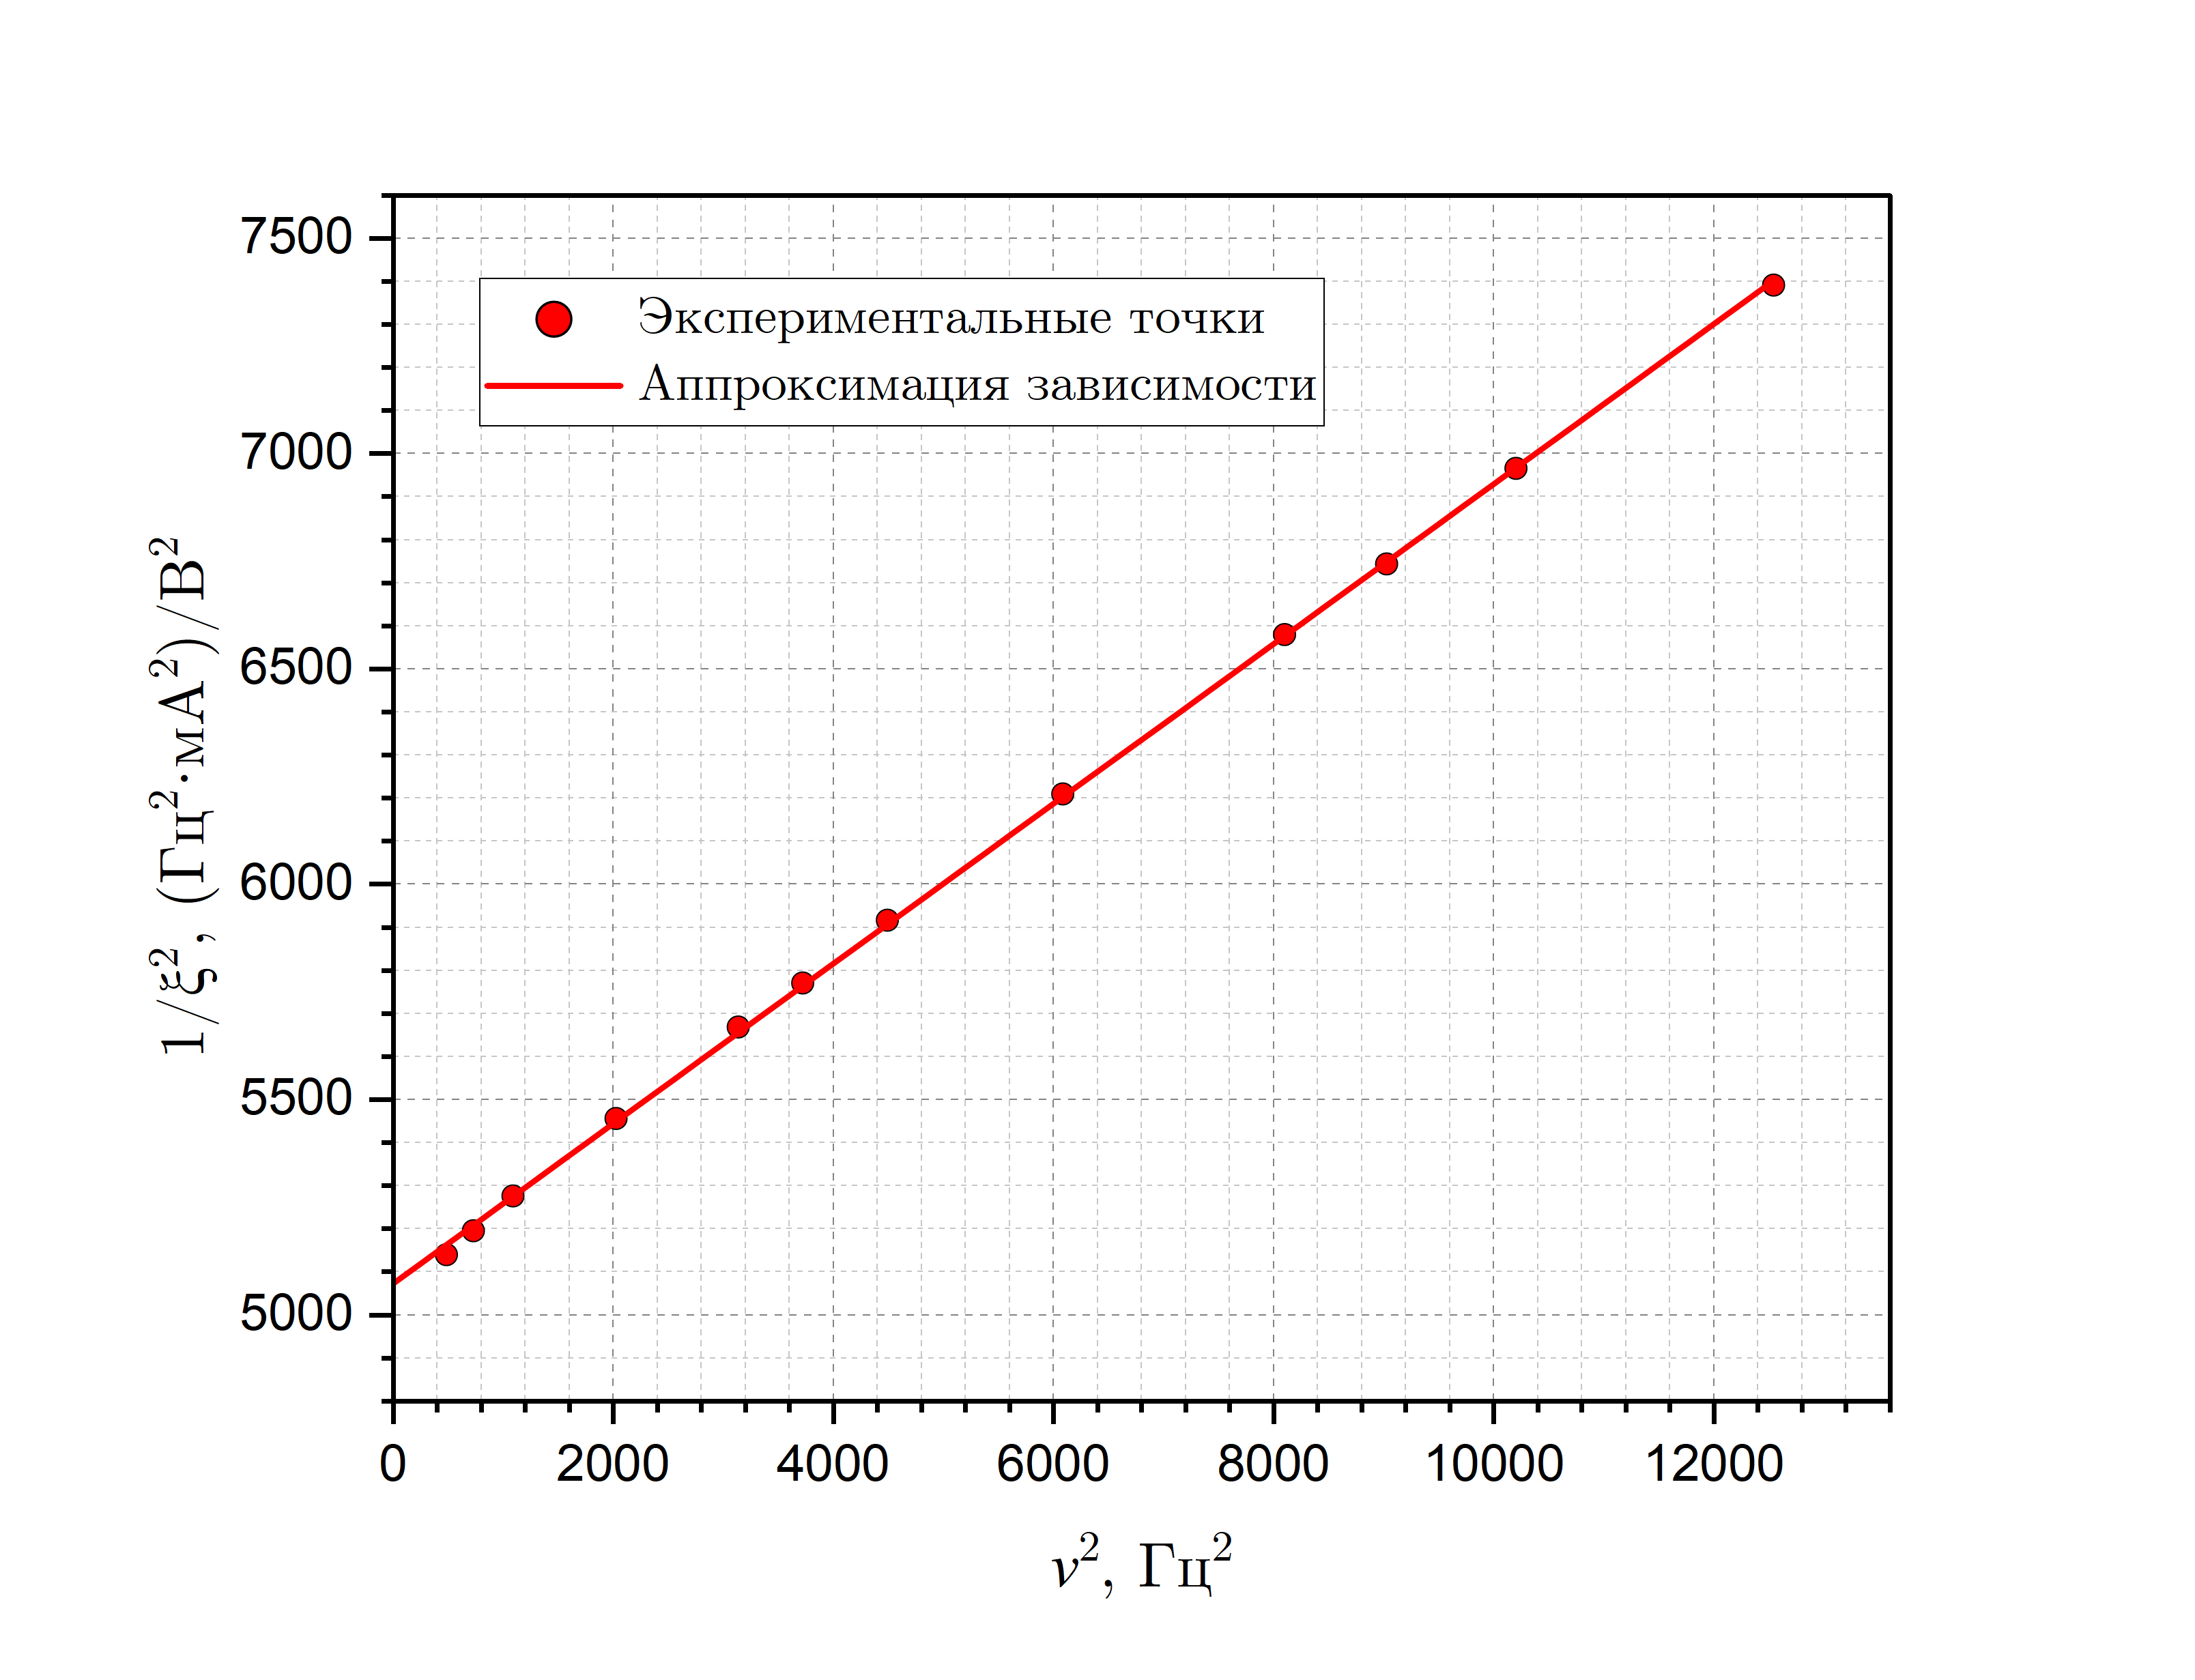
\includegraphics[width = 14 cm]{images/graph_xi.png}
        \caption{График зависимости $1/\xi^2 = f(\nu^2)$}
        \label{graph:xi}
    \end{figure}

    В области низких частот ($\nu \ll \nu_h$) из соотношения (\ref{eq:nu_ll_2}), получим

    \begin{equation*}
        \frac{\xi^2}{\xi_0^2} = \frac{1}{1 + \pi^2 a^2 h^2 \sigma^2 \mu_0^2 \nu^2} \Rightarrow \frac{1}{\xi^2} = k^2 \nu^2 + \frac{1}{\xi_0^2}.
    \end{equation*}

     Аппроксимируя полученные данные при помощи программы \textit{OriginPro 2023b}, получим

     \begin{equation*}
         k^2 = \left( 0,1857 \pm 0,0008 \right) \frac{\text{мА}^2}{\text{В}^2} \Rightarrow k = \left( 0,431 \pm 0,002 \right) \frac{\text{мА}}{\text{В}},
     \end{equation*}

     \begin{equation*}
         \frac{1}{\xi_0^2} = \left( 5073 \pm 5 \right) \frac{\text{Гц}^2 \cdot \text{мА}^2}{\text{В}^2} \Rightarrow \frac{1}{\xi_0} = \left( 71,22 \pm 0,04 \right) \frac{\text{Гц} \cdot \text{мА}}{\text{В}}.
     \end{equation*}

     Отсюда,

     \begin{equation*}
         \boxed{\sigma = \frac{k}{\pi \frac{\mu_0 }{\xi_0}ah} = \left( 4,542 \pm 0,005 \right) \cdot 10^7 \text{ См/м}}.
     \end{equation*}

     \subsection{Измерение проводимости через разность фаз в низкочастотном диапазоне}

     В этом пункте была исследована зависимость величины $\xi$ и фазового сдвига $\psi$ от частоты $\nu$ при низких частотах в диапазоне от $0,01 \nu_h$ до $\sim 0,5 \nu_h$. Результаты измерений представлены в таблице \ref{table:phase_ll}.

     \begin{table}[H]
        \centering
        \begin{tabular}{|c|c|c|c|c|c|c|c|}
        \hline
        $\nu$, Гц & $x$, дел & $x_0$, дел & $\Delta x$, дел. & $\psi$, рад. & $\Delta \psi$, рад. & $\tg \psi$ & $\Delta \tg \psi$ \\ \hline
        100 & 17 & 25 & \multirow{20}{*}{1} & 0,57 & 0,04 & 0,63 & 0,06 \\ \cline{1-3} \cline{5-8} 
        112 & 16 & 23 &  & 0,61 & 0,05 & 0,71 & 0,07 \\ \cline{1-3} \cline{5-8} 
        123 & 14 & 20 &  & 0,63 & 0,05 & 0,73 & 0,08 \\ \cline{1-3} \cline{5-8} 
        135 & 14 & 19 &  & 0,74 & 0,07 & 0,92 & 0,12 \\ \cline{1-3} \cline{5-8} 
        146 & 13 & 18 &  & 0,70 & 0,07 & 0,84 & 0,11 \\ \cline{1-3} \cline{5-8} 
        157 & 24 & 33 &  & 0,71 & 0,04 & 0,87 & 0,06 \\ \cline{1-3} \cline{5-8} 
        168 & 24 & 32 &  & 0,79 & 0,04 & 1,00 & 0,08 \\ \cline{1-3} \cline{5-8} 
        180 & 19 & 25 &  & 0,82 & 0,05 & 1,06 & 0,12 \\ \cline{1-3} \cline{5-8} 
        191 & 20 & 26 &  & 0,85 & 0,05 & 1,13 & 0,12 \\ \cline{1-3} \cline{5-8} 
        202 & 18 & 23 &  & 0,89 & 0,06 & 1,23 & 0,16 \\ \cline{1-3} \cline{5-8} 
        213 & 19 & 24 &  & 0,92 & 0,06 & 1,30 & 0,17 \\ \cline{1-3} \cline{5-8} 
        225 & 20 & 25 &  & 0,94 & 0,06 & 1,38 & 0,17 \\ \cline{1-3} \cline{5-8} 
        337 & 26 & 30 &  & 1,15 & 0,06 & 2,25 & 0,35 \\ \cline{1-3} \cline{5-8} 
        450 & 21 & 24 &  & 1,18 & 0,07 & 2,41 & 0,51 \\ \cline{1-3} \cline{5-8} 
        562 & 19 & 21 &  & 1,27 & 0,09 & 3,24 & 1,04 \\ \cline{1-3} \cline{5-8} 
        675 & 20 & 22 &  & 1,29 & 0,09 & 3,41 & 1,09 \\ \cline{1-3} \cline{5-8} 
        788 & 16 & 16 &  & 1,57 & $\infty$ & - & - \\ \cline{1-3} \cline{5-8} 
        900 & 14 & 14 &  & 1,57 & $\infty$ & - & - \\ \cline{1-3} \cline{5-8} 
        1013 & 12 & 12 & & 1,57 & $\infty$ & - & - \\ \cline{1-3} \cline{5-8} 
        1125 & 11 & 11 & & 1,57 & $\infty$ & - & - \\ \hline
        \end{tabular}
        \caption{Результаты измерения зависимости $\psi (\nu)$}
        \label{table:phase_ll}
    \end{table}

    По этим данным построим график зависимости $\tg \psi = f(\nu)$ (рис. \ref{graph:tg_psi}).

    \begin{figure}[H]
        \centering
        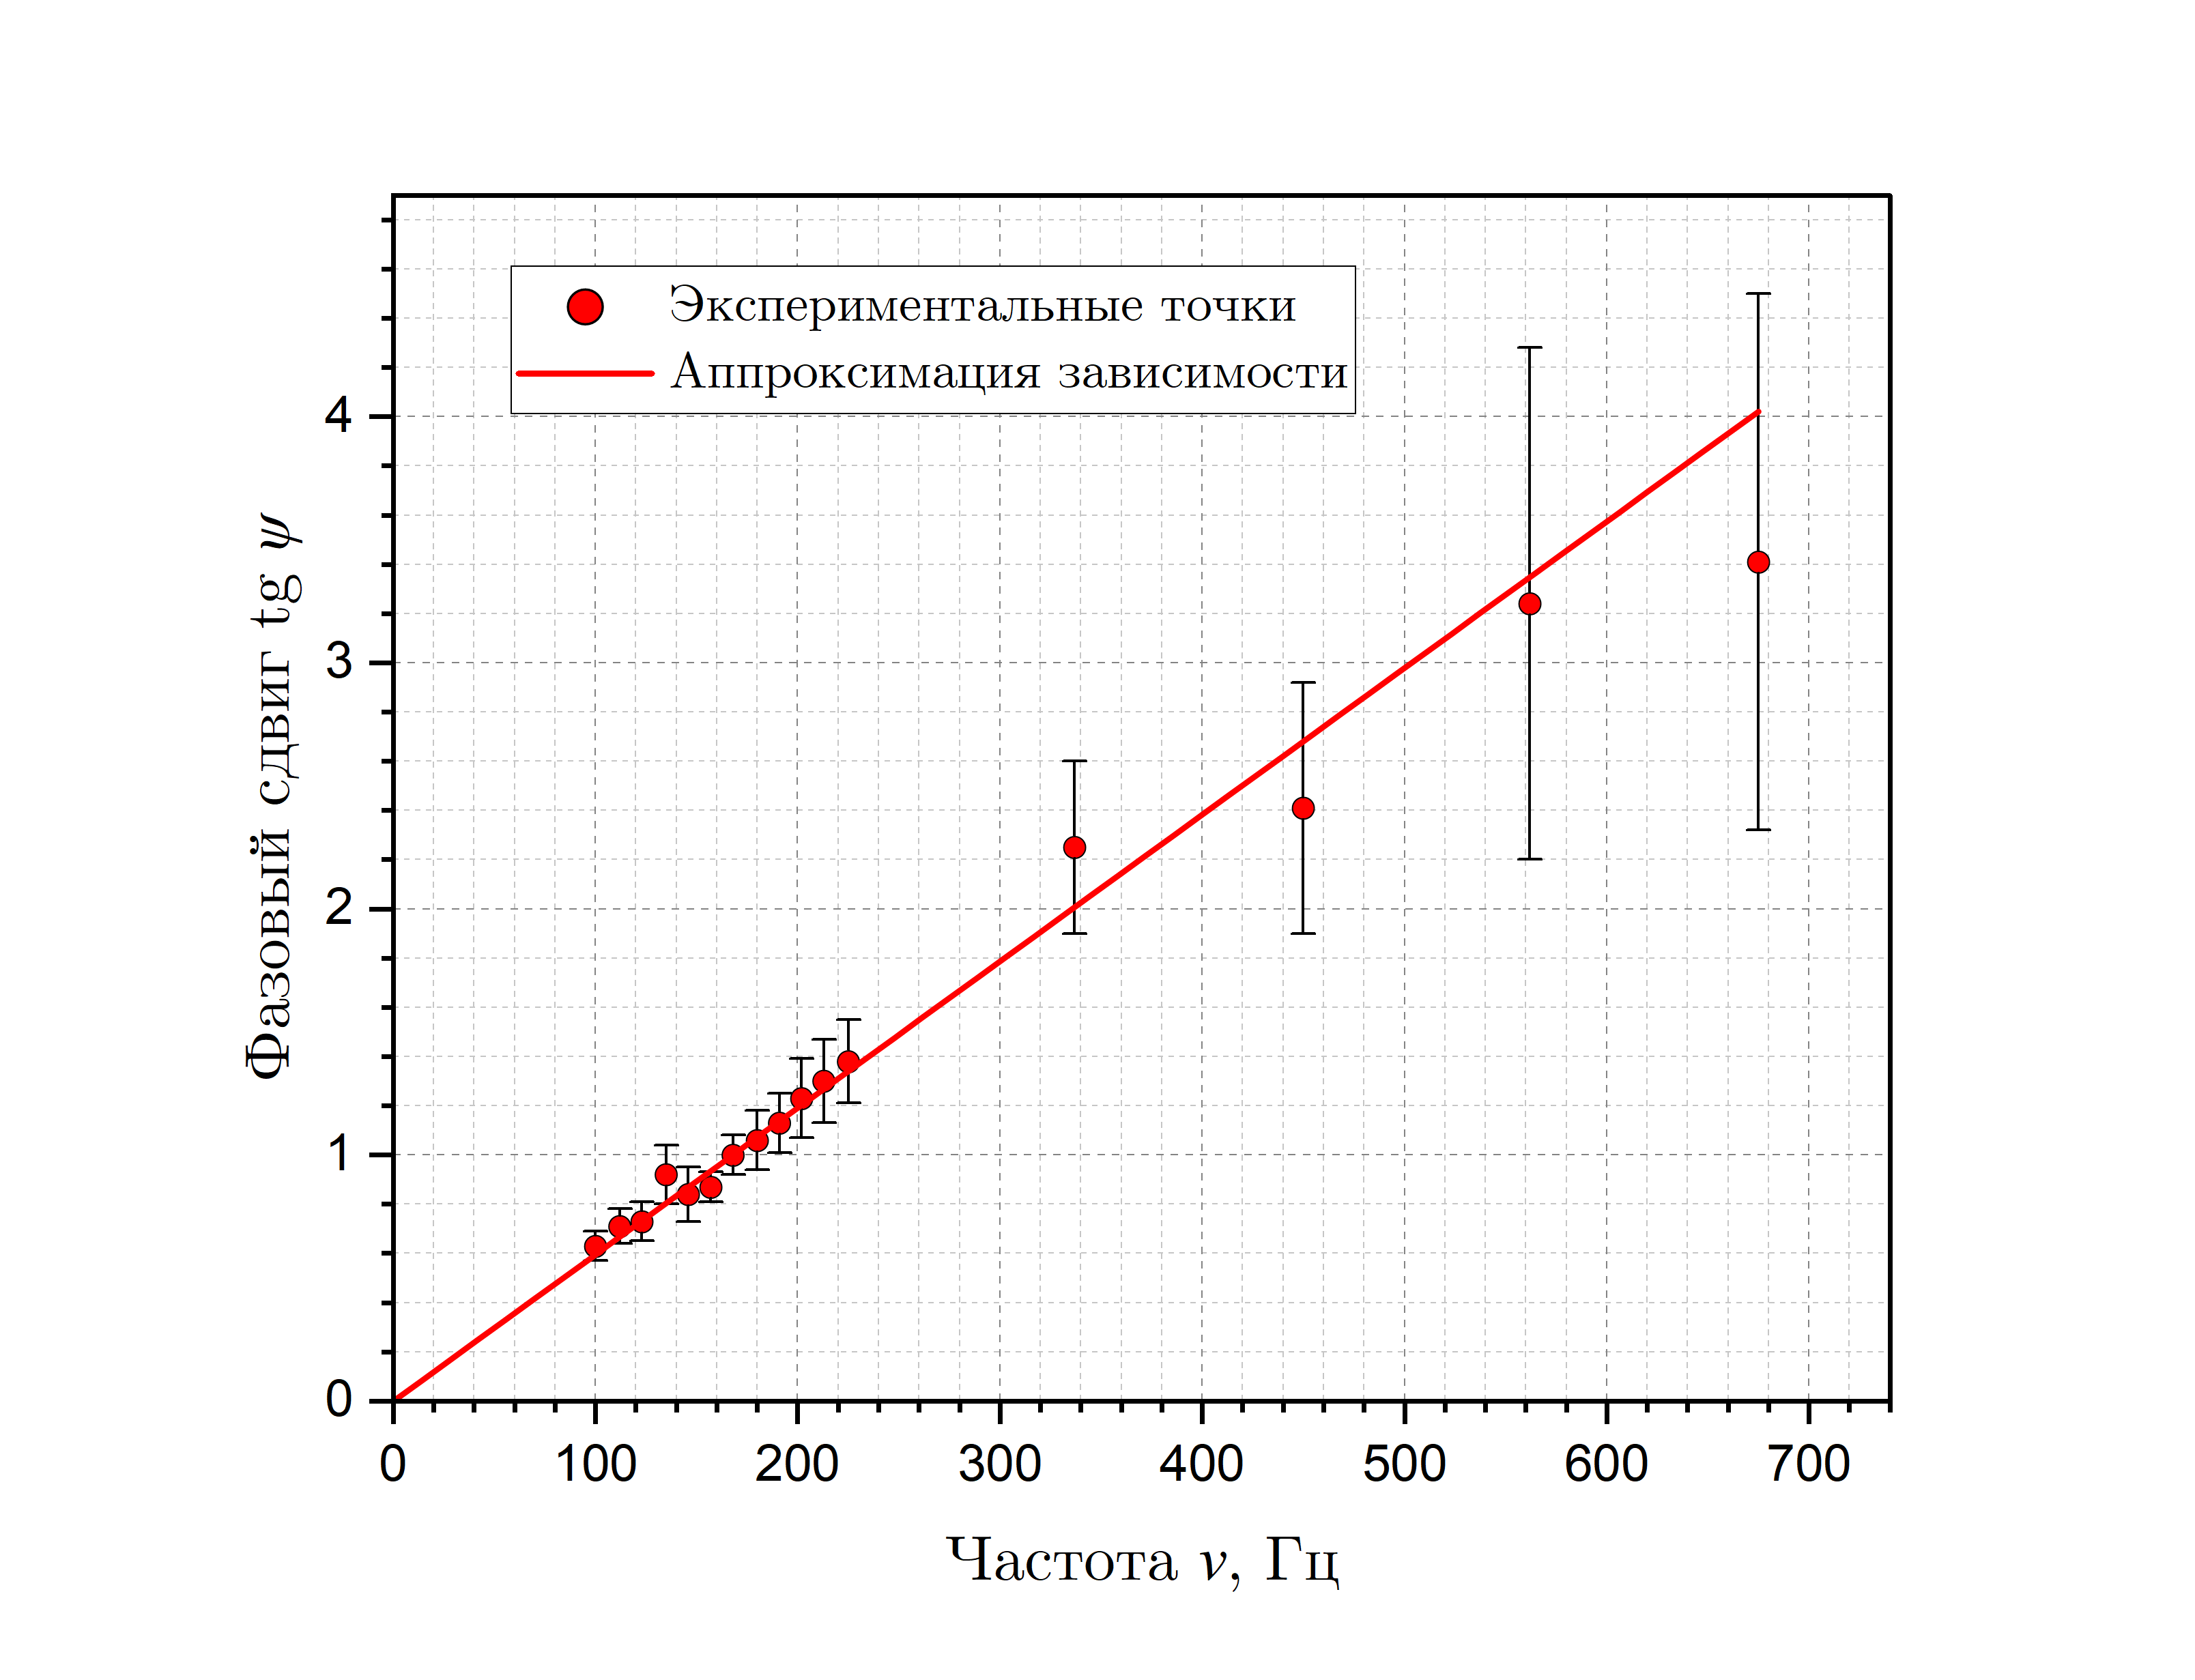
\includegraphics[width = 14 cm]{images/graph_tg_psi.png}
        \caption{График зависимости $\tg \psi = f(\nu)$}
        \label{graph:tg_psi}
    \end{figure}

    Аппроксимируя полученные данные при помощи программы \textit{OriginPro 2023b}, получим 

    \begin{equation*}
        k = \frac{d(\tg \psi)}{d \nu} = \left( 0,00596 \pm 0,00009 \right) \text{ Гц}^{-1}.
    \end{equation*}

    Отсюда,

    \begin{equation*}
        \boxed{\sigma = \frac{k}{\pi \mu_0 ah} = \left( 4,47 \pm 0,07 \right) \cdot 10^7 \text{ См/м}}.
    \end{equation*}

    \subsection{Измерение проводимости через разность фаз в высокочастотном диапазоне}

    Была исследована зависимость величины $\xi$ и фазового сдвига $\psi$ от частоты $\nu$ при высоких частотах в диапазоне от $0,5 \nu_h$ до $\sim 15 \nu_h$. Результаты измерений представлены в таблице \ref{table:phase_gg}.

    \begin{table}[H]
        \centering
        \begin{tabular}{|c|c|c|c|c|c|c|}
        \hline
        $\nu$, Гц & $\sqrt{\nu}$, $\text{Гц}^{0,5}$ & $x$, дел. & $x_0$, дел. & $\delta x$, дел. & $\psi - \pi/4$ & $\Delta \psi$ \\ \hline
        100 & 10,00 & 17 & 25 & \multirow{30}{*}{1} & -0,22 & 0,02 \\ \cline{1-4} \cline{6-7} 
        112 & 10,58 & 16 & 23 &  & -0,17 & 0,01 \\ \cline{1-4} \cline{6-7} 
        123 & 11,09 & 14 & 20 &  & -0,16 & 0,01 \\ \cline{1-4} \cline{6-7} 
        135 & 11,62 & 14 & 19 &  & -0,04 & 0,01 \\ \cline{1-4} \cline{6-7} 
        146 & 12,08 & 13 & 18 &  & -0,09 & 0,01 \\ \cline{1-4} \cline{6-7} 
        157 & 12,53 & 24 & 33 &  & -0,07 & 0,01 \\ \cline{1-4} \cline{6-7} 
        168 & 12,96 & 24 & 32 &  & 0,00 & 0,01 \\ \cline{1-4} \cline{6-7} 
        180 & 13,42 & 19 & 25 &  & 0,03 & 0,01 \\ \cline{1-4} \cline{6-7} 
        191 & 13,82 & 20 & 26 &  & 0,06 & 0,01 \\ \cline{1-4} \cline{6-7} 
        202 & 14,21 & 18 & 23 &  & 0,10 & 0,01 \\ \cline{1-4} \cline{6-7} 
        213 & 14,59 & 19 & 24 &  & 0,13 & 0,01 \\ \cline{1-4} \cline{6-7} 
        225 & 15,00 & 20 & 25 &  & 0,16 & 0,01 \\ \cline{1-4} \cline{6-7} 
        337 & 18,36 & 26 & 30 &  & 0,37 & 0,02 \\ \cline{1-4} \cline{6-7} 
        450 & 21,21 & 21 & 24 &  & 0,39 & 0,02 \\ \cline{1-4} \cline{6-7} 
        562 & 23,71 & 19 & 21 &  & 0,49 & 0,03 \\ \cline{1-4} \cline{6-7} 
        675 & 25,98 & 20 & 22 &  & 0,50 & 0,03 \\ \cline{1-4} \cline{6-7} 
        2000 & 44,72 & 13 & 13 &  & 0,79 & 0,09 \\ \cline{1-4} \cline{6-7} 
        3377 & 58,11 & 17 & 15 &  & 1,20 & 0,11 \\ \cline{1-4} \cline{6-7} 
        4000 & 63,25 & 15 & 12 &  & 1,57 & 0,17 \\ \cline{1-4} \cline{6-7} 
        5628 & 75,02 & 11 & 9 &  & 1,48 & 0,21 \\ \cline{1-4} \cline{6-7} 
        6500 & 80,62 & 10 & 8 &  & 1,57 & 0,25 \\ \cline{1-4} \cline{6-7} 
        7880 & 88,77 & 21 & 16 &  & 1,77 & 0,14 \\ \cline{1-4} \cline{6-7} 
        8500 & 92,20 & 20 & 14 &  & 2,13 & 0,19 \\ \cline{1-4} \cline{6-7} 
        10132 & 100,66 & 18 & 13 &  & 1,99 & 0,19 \\ \cline{1-4} \cline{6-7} 
        12383 & 111,28 & 15 & 10 &  & 2,36 & 0,28 \\ \cline{1-4} \cline{6-7} 
        14635 & 120,98 & 14 & 9 &  & 2,53 & 0,33 \\ \cline{1-4} \cline{6-7} 
        16886 & 129,95 & 24 & 15 &  & 2,67 & 0,21 \\ \cline{1-4} \cline{6-7} 
        19138 & 138,34 & 22 & 13 &  & 2,96 & 0,26 \\ \cline{1-4} \cline{6-7} 
        21390 & 146,25 & 19 & 11 &  & 3,07 & 0,32 \\ \cline{1-4} \cline{6-7} 
        23641 & 153,76 & 20 & 11 &  & 3,36 & 0,35 \\ \hline
        \end{tabular}
        \caption{Результаты измерения зависимости $\psi - \pi/4(\sqrt{\nu})$}
        \label{table:phase_gg}
    \end{table}

    По этим данным построим график зависимости $\psi - \pi/4 = f(\sqrt{\nu})$ (рис. \ref{graph:psi}).

    \begin{figure}[H]
        \centering
        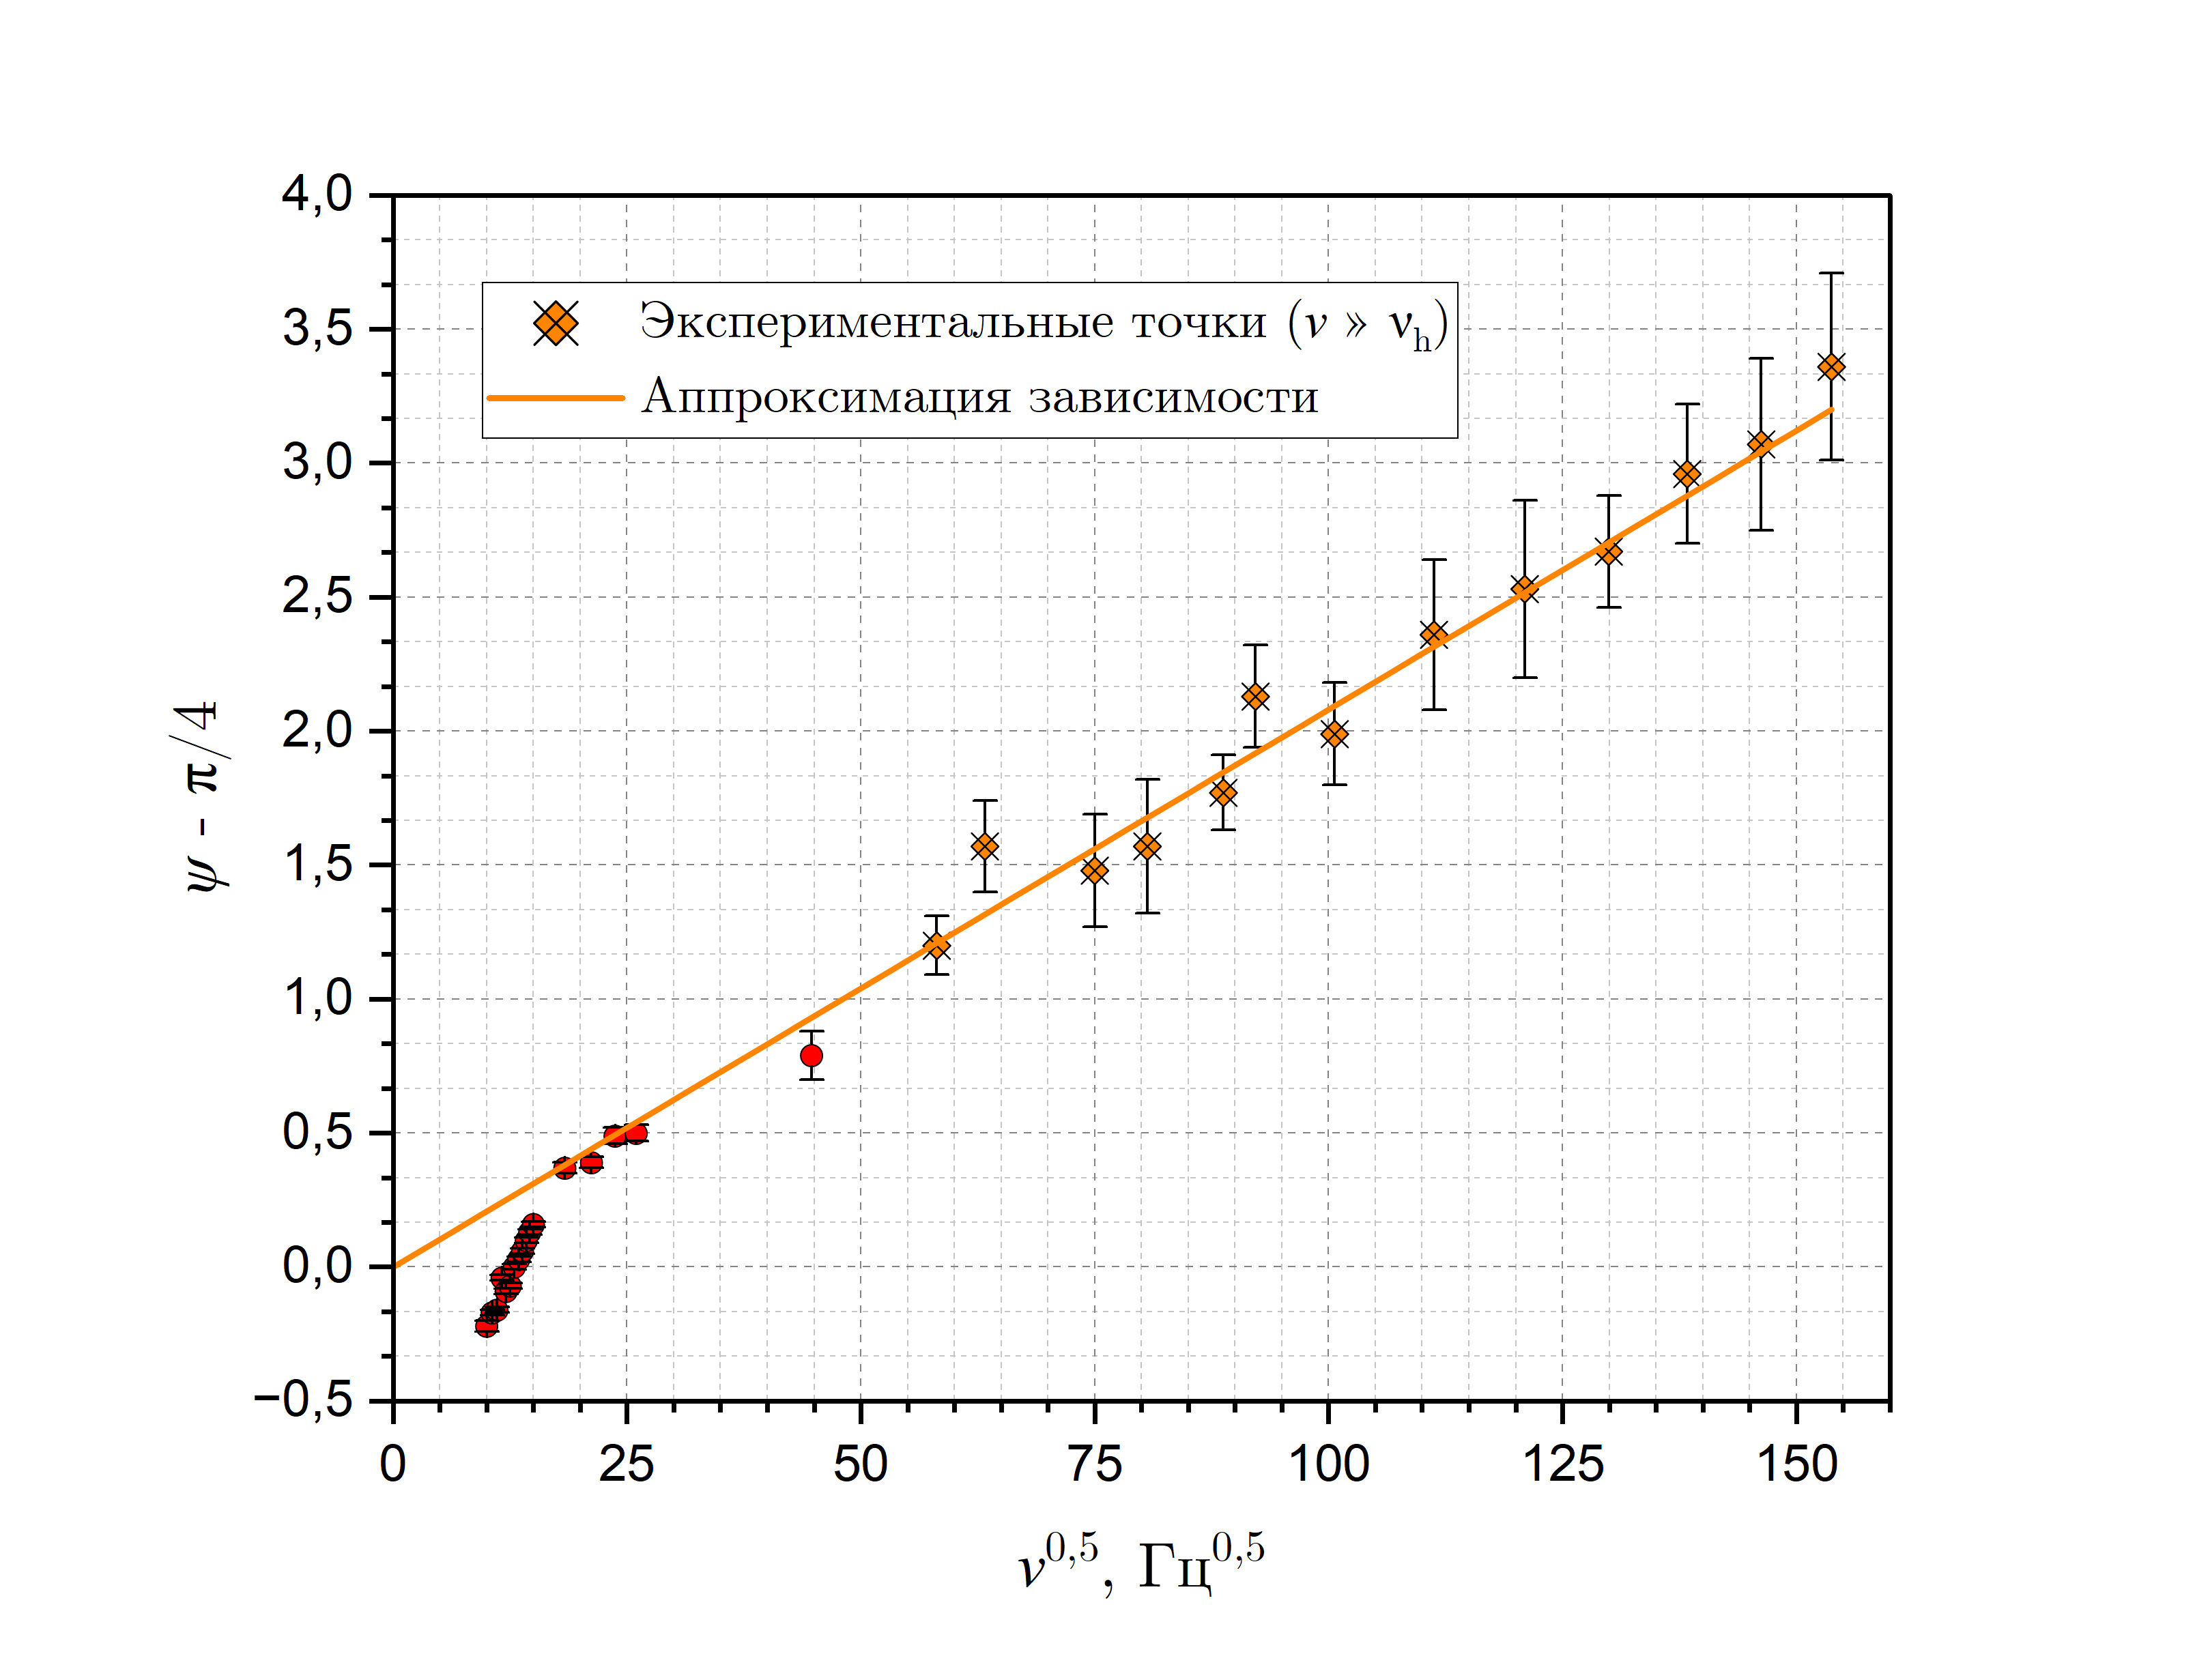
\includegraphics[width = 14 cm]{images/graph_psi.png}
        \caption{График зависимости $\psi - \pi/4 = f(\sqrt{\nu})$}
        \label{graph:psi}
    \end{figure}

    Аппроксимируя полученные данные при помощи программы \textit{OriginPro 2023b}, получим 

    \begin{equation*}
        k = \frac{d(\psi - \pi/4)}{d(\sqrt{\nu})} = \left( 0,0208 \pm 0,0003 \right) \text{ Гц}^{-0,5}.
    \end{equation*}

    Отсюда,

    \begin{equation*}
        \boxed{\sigma = \frac{k^2}{h^2 \pi \mu_0} = \left( 4,87 \pm 0,09 \right) \cdot 10^7 \text{ См/м}}.
    \end{equation*}

    \subsection{Измерение проводимости через изменение индуктивности}

    Была исследована зависимость индуктивности катушки $L$ от частоты $\nu$. Результаты измерений приведены в таблице \ref{table:inductivity}. 

    По этим данным построим график зависимости $L (\nu)$ (рис. \ref{graph:L_nu}), определим и занесём в таблицу \ref{table:inductivity} максимальное и минимальное значения индуктивности.


    \begin{figure}[H]
        \centering
        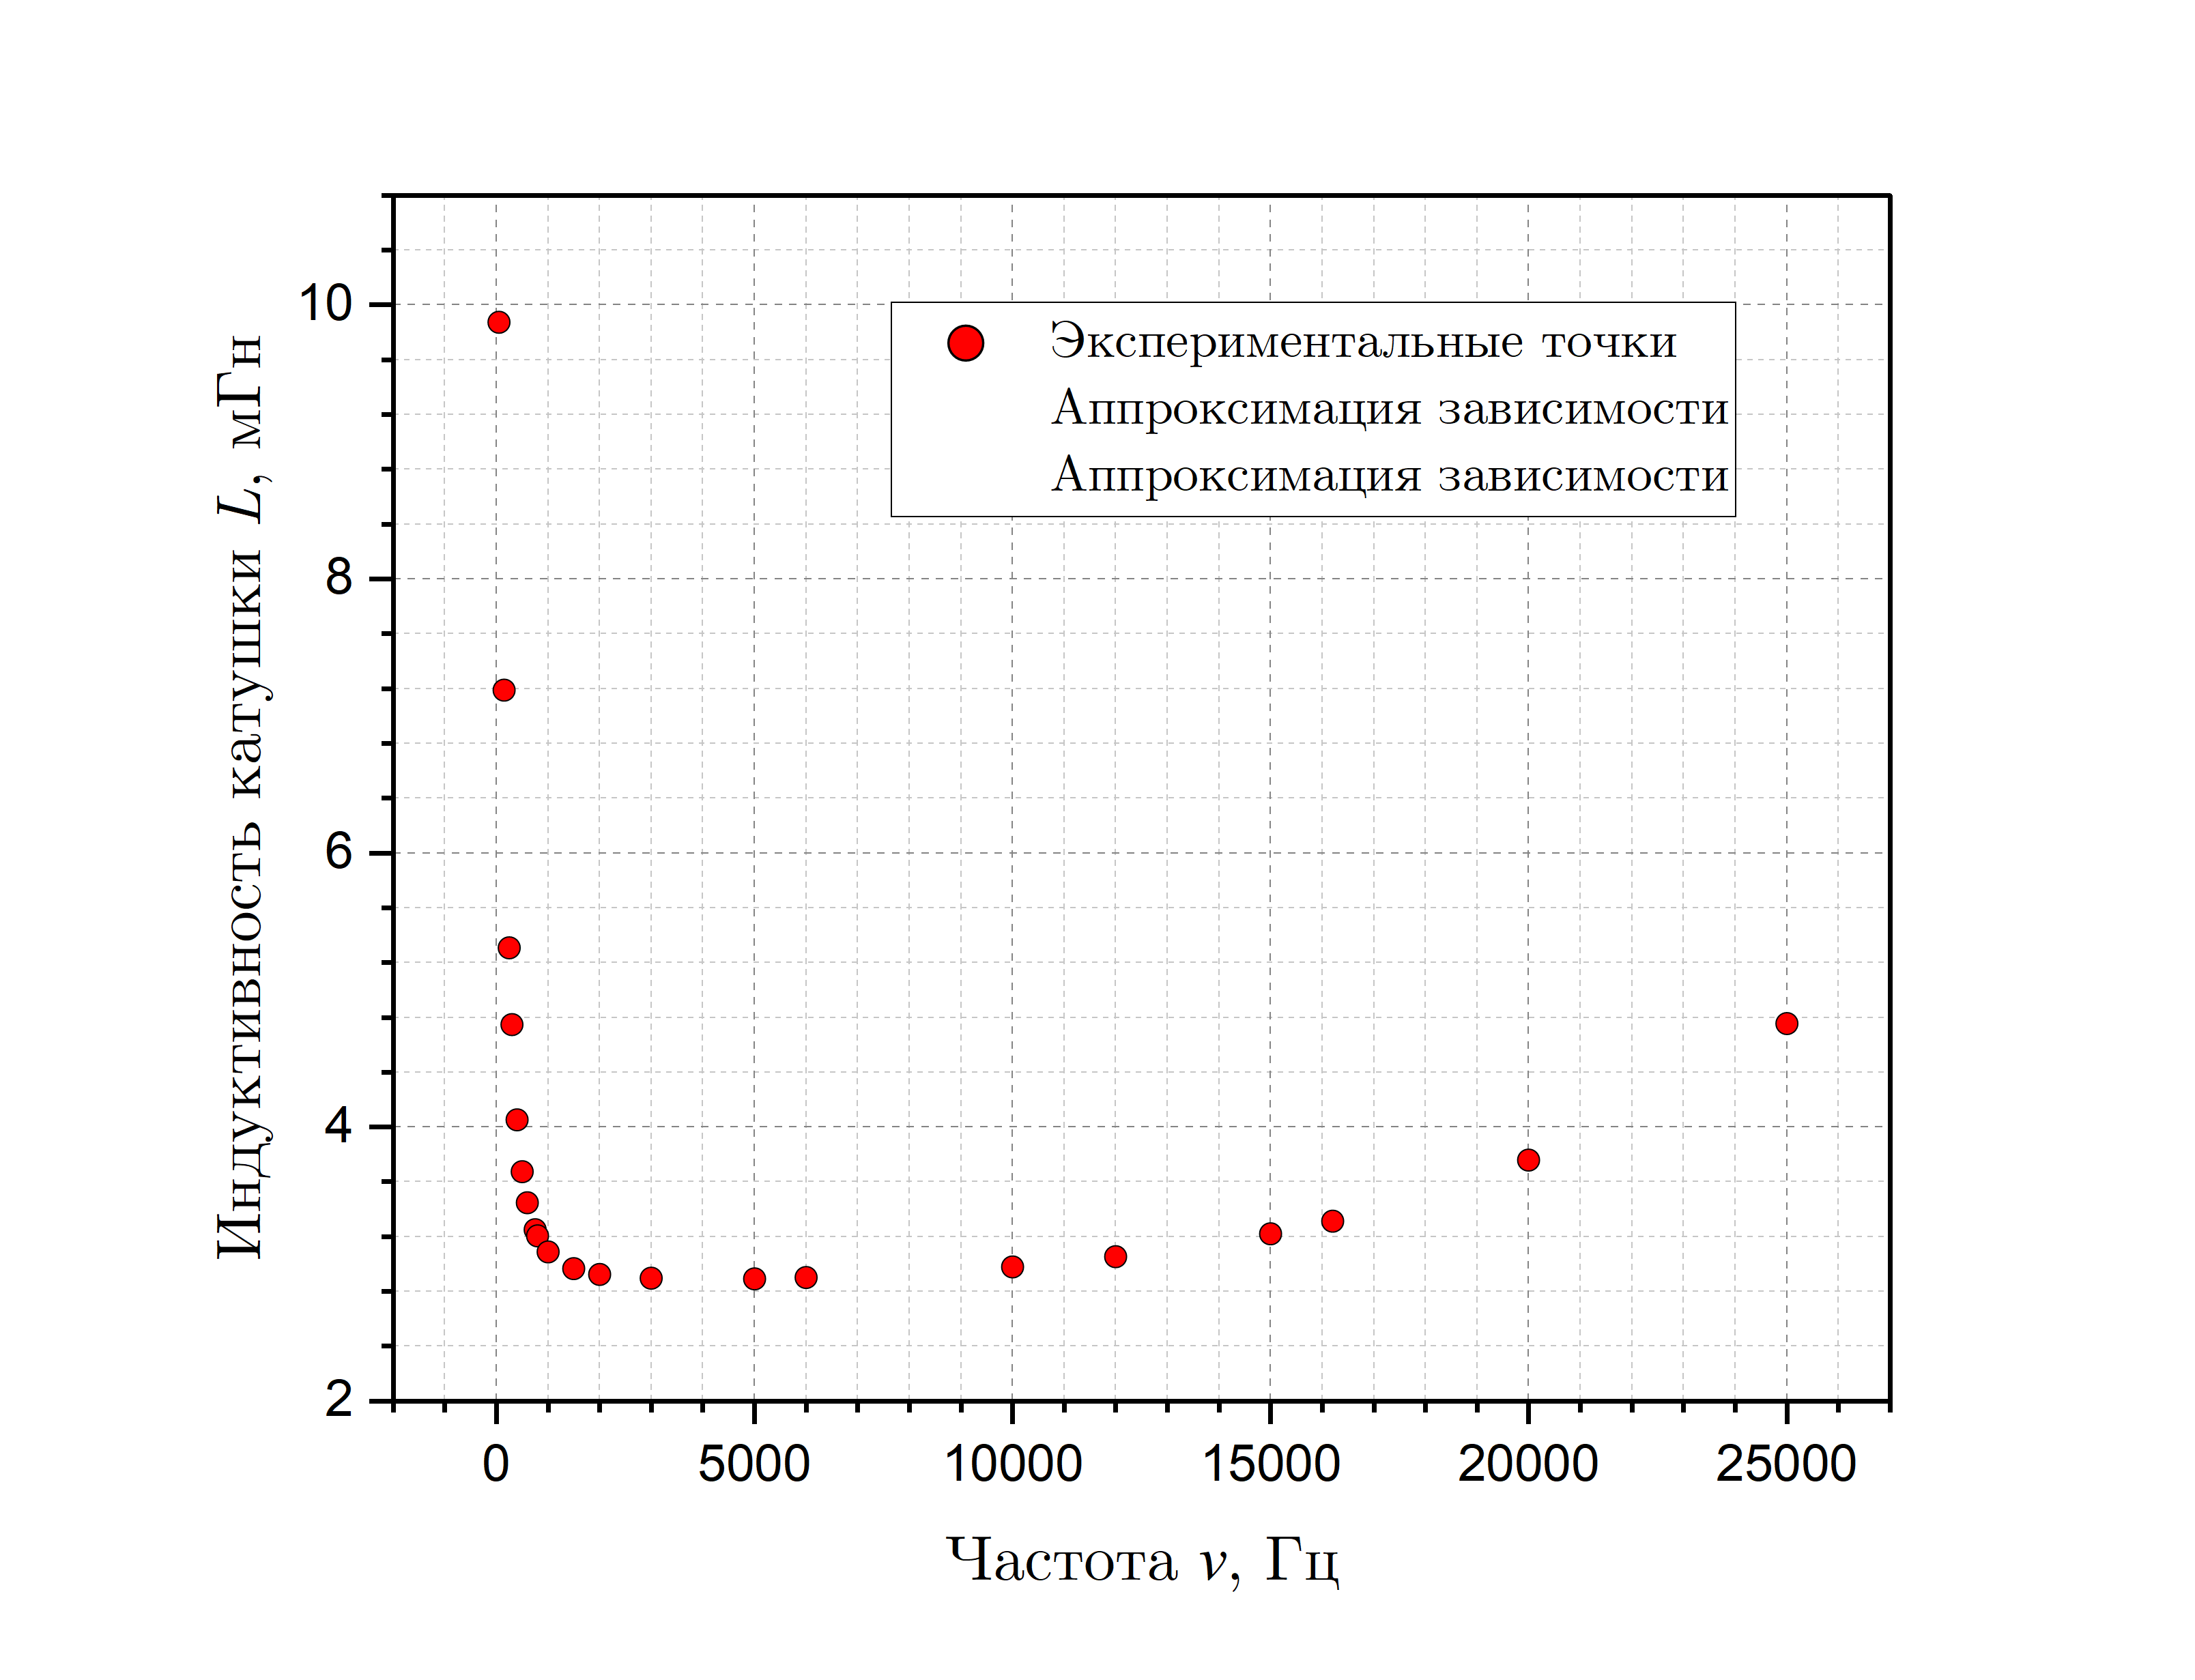
\includegraphics[width = 14 cm]{images/graph_l_nu.png}
        \caption{График зависимости $L (\nu)$}
        \label{graph:L_nu}
    \end{figure}

    \begin{table}[H]
        \centering
        \begin{tabular}{|c|c|c|c|c|c|}
        \hline
        $\nu$, Гц & $\nu^2$, $\text{кГц}^2$ & $L$, мГн & $L_{max}$, мГн &$L_{min}$, мГн & $(L_{max} - L) / (L - L_{min})$ \\ \hline
        50 & 0,0025 & 9,8733 & \multirow{21}{*}{9,8733} & \multirow{21}{*}{2,8938} & 0,0000 \\ \cline{1-3} \cline{6-6} 
        150 & 0,0225 & 7,1898 &  &  & 0,6247 \\ \cline{1-3} \cline{6-6} 
        250 & 0,0625 & 5,3095 &  &  & 1,8892 \\ \cline{1-3} \cline{6-6} 
        300 & 0,0900 & 4,7488 &  &  & 2,7625 \\ \cline{1-3} \cline{6-6} 
        400 & 0,1600 & 4,0547 &  &  & 5,0121 \\ \cline{1-3} \cline{6-6} 
        500 & 0,2500 & 3,6753 &  &  & 7,9309 \\ \cline{1-3} \cline{6-6} 
        600 & 0,3600 & 3,4495 &  &  & 11,5598 \\ \cline{1-3} \cline{6-6} 
        750 & 0,5625 & 3,2521 &  &  & 18,4795 \\ \cline{1-3} \cline{6-6} 
        800 & 0,6400 & 3,2086 &  &  & 21,1712 \\ \cline{1-3} \cline{6-6} 
        1000 & 1,0000 & 3,0903 &  &  & 34,5191 \\ \cline{1-3} \cline{6-6} 
        1500 & 2,2500 & 2,9681 &  &  & 92,9367 \\ \cline{1-3} \cline{6-6} 
        2000 & 4,0000 & 2,9259 &  &  & 216,4299 \\ \cline{1-3} \cline{6-6} 
        3000 & 9,0000 & 2,8982 &  &  & 1585,2500 \\ \cline{1-3} \cline{6-6} 
        5000 & 25,0000 & 2,8938 &  &  & NaN \\ \cline{1-3} \cline{6-6} 
        6000 & 36,0000 & 2,903 &  &  & 757,6413 \\ \cline{1-3} \cline{6-6} 
        10000 & 100,0000 & 2,981 &  &  & 79,0401 \\ \cline{1-3} \cline{6-6} 
        12000 & 144,0000 & 3,0557 &  &  & 42,1099 \\ \cline{1-3} \cline{6-6} 
        15000 & 225,0000 & 3,2234 &  &  & 20,1757 \\ \cline{1-3} \cline{6-6} 
        16200 & 262,4400 & 3,3139 &  &  & 15,6139 \\ \cline{1-3} \cline{6-6} 
        20000 & 400,0000 & 3,7614 &  &  & 7,0446 \\ \cline{1-3} \cline{6-6} 
        25000 & 625,0000 & 4,7573 &  &  & 2,7454 \\ \hline
        \end{tabular}
        \caption{Результаты измерения зависимости $L(\nu)$ и $(L_{max} - L) / (L - L_{min}) = f(\nu^2)$}
        \label{table:inductivity}
    \end{table}

    Теперь построим график зависимости $(L_{max} - L) / (L - L_{min}) = f(\nu^2)$, пользуясь таблицей \ref{table:inductivity}. Полученный график изображён на рис. \ref{graph:rel_l_nu}.

     \begin{figure}[H]
        \centering
        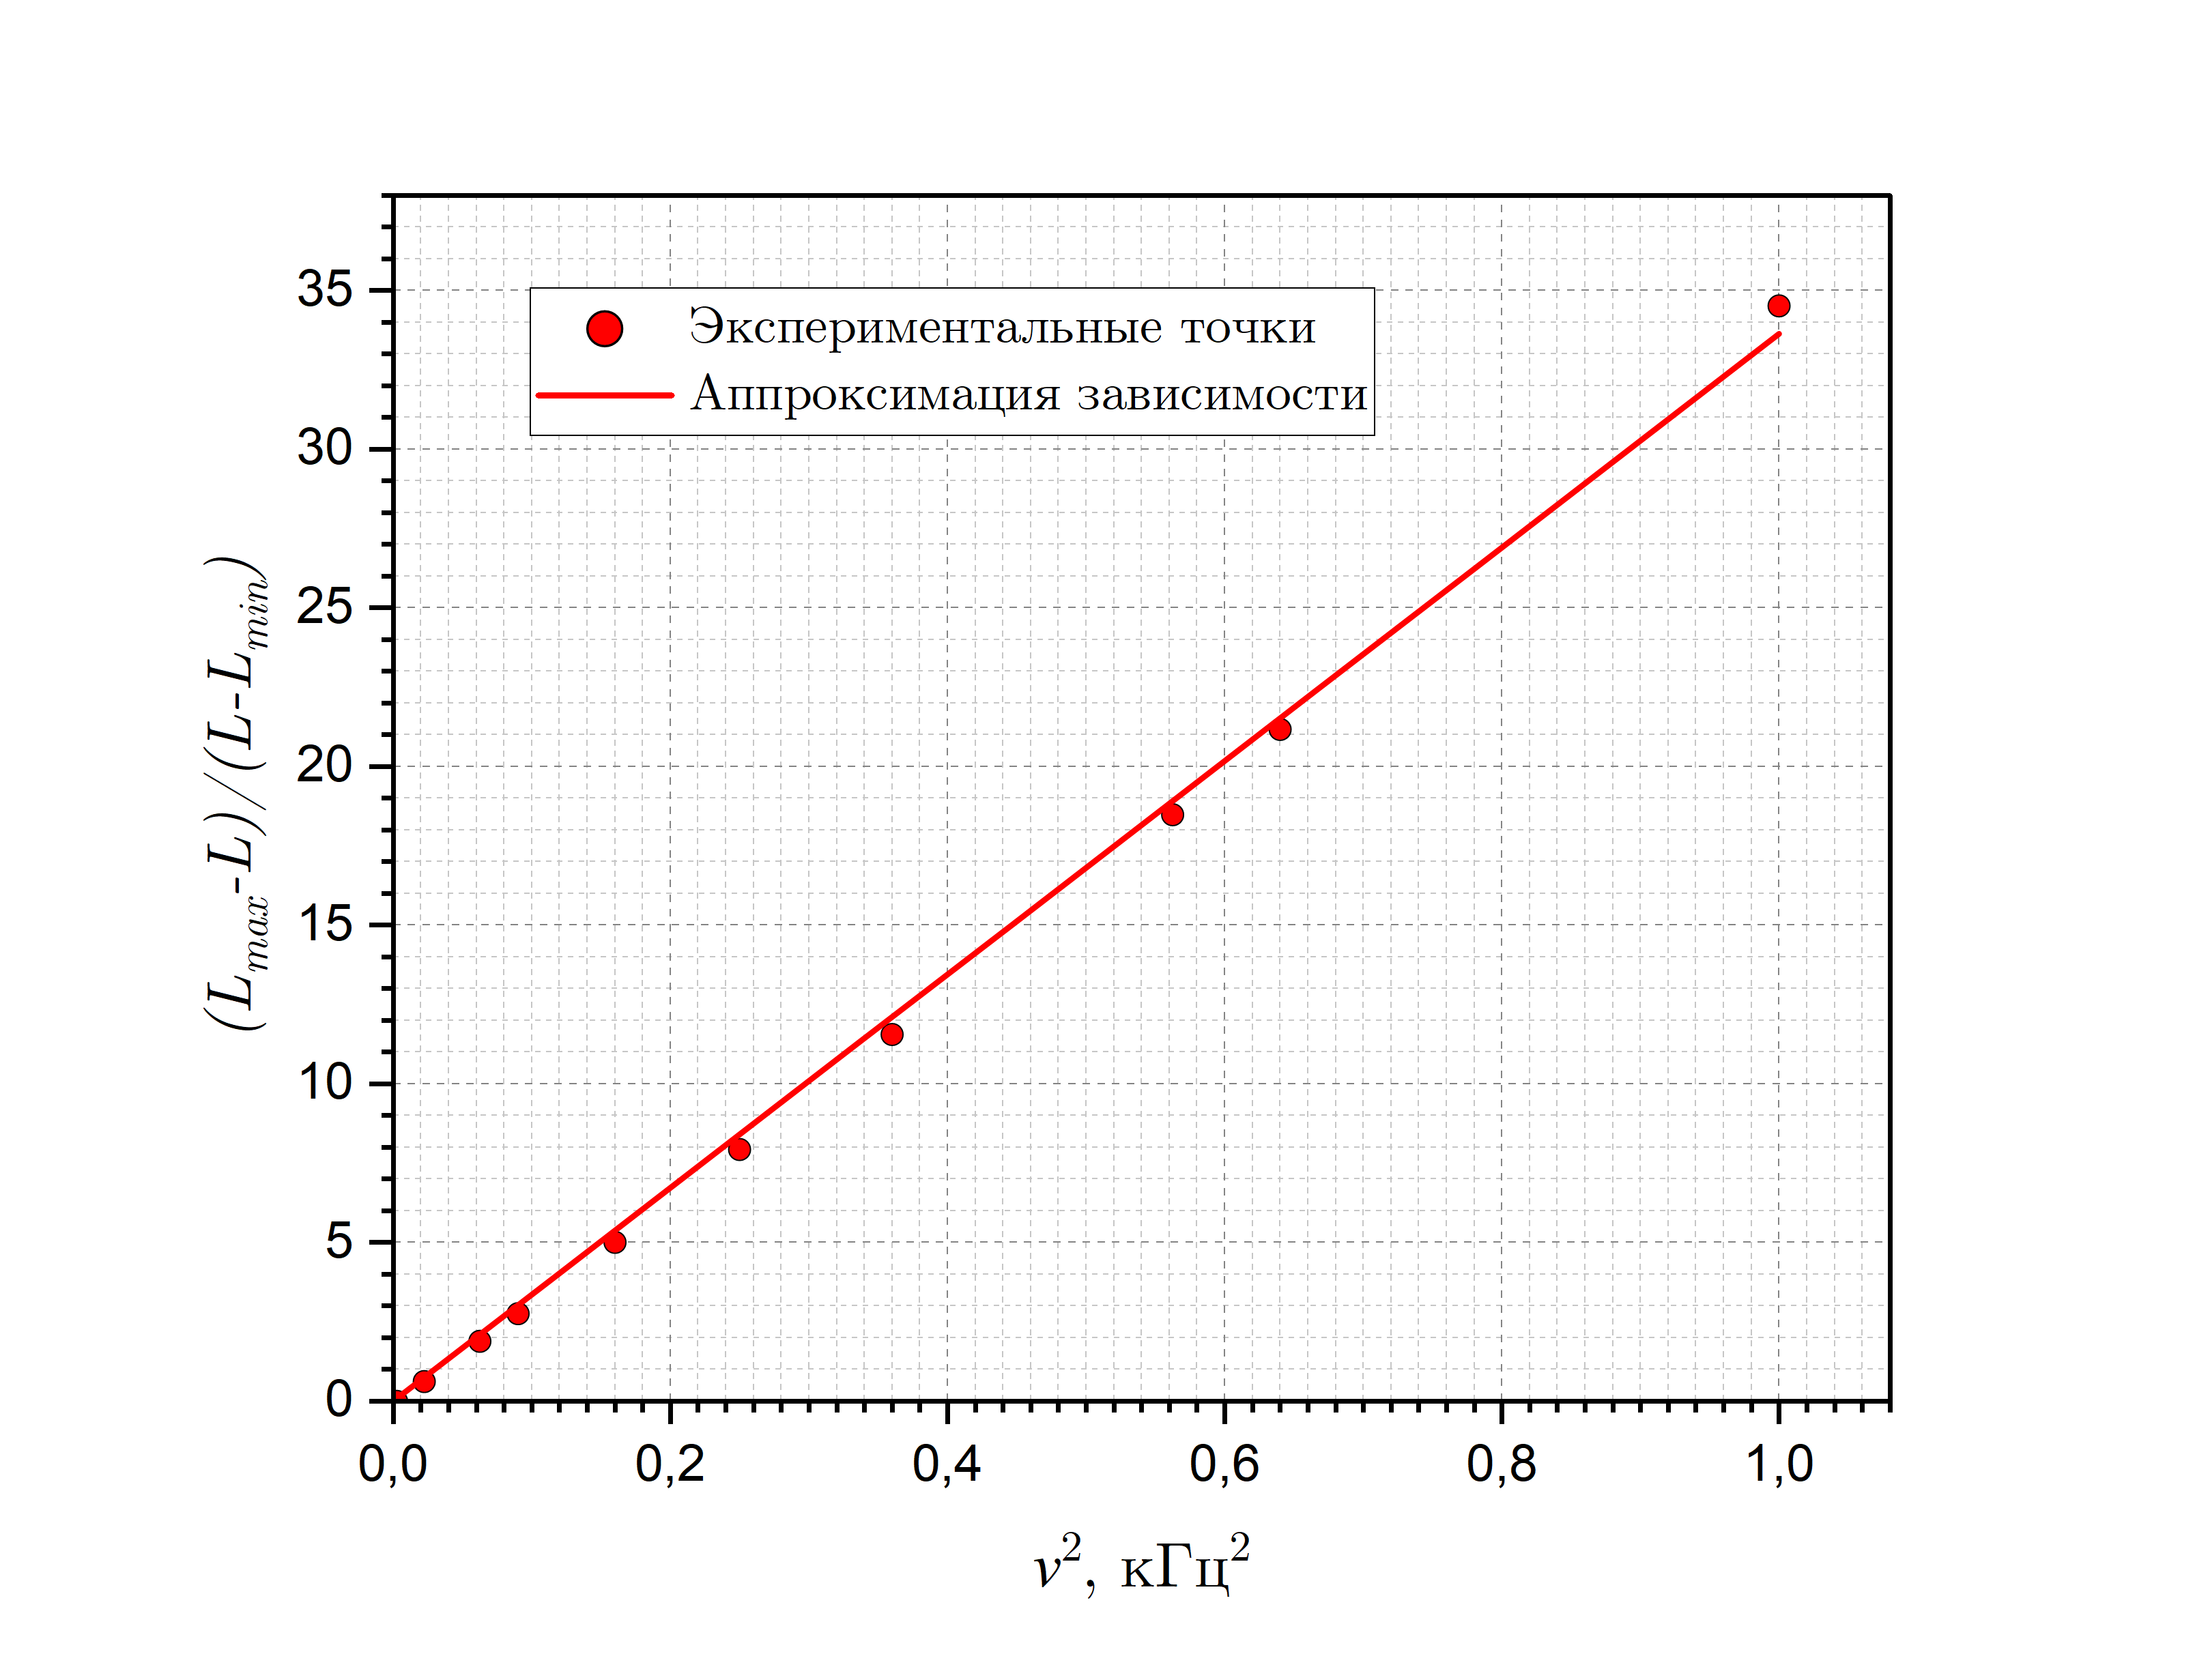
\includegraphics[width = 14 cm]{images/graph_rel_l_nu.png}
        \caption{График зависимости $(L_{max} - L) / (L - L_{min}) = f(\nu^2)$}
        \label{graph:rel_l_nu}
    \end{figure}

    Аппроксимируя полученные данные при помощи программы \textit{OriginPro 2023b}, получим 

    \begin{equation*}
        k = \frac{d((L_{max} - L) / (L - L_{min}))}{d(\nu^2)} = \left( 33,6 \pm 0,3 \right) \text{ кГц}^{-2}.
    \end{equation*}

    Отсюда,

    \begin{equation*}
        \boxed{\sigma = \frac{\sqrt{k}}{\pi ah \mu_0} = \left( 4,35 \pm 0,02 \right) \cdot 10^7 \text{ См/м}}.
    \end{equation*}

    \subsection{Исследование коэффициентов ослабления поля}

        Используя значение $\xi_0$, полученное ранее, расчитаем зависимость коэффициентов ослабления поля для всего диапазона частот, полученных в ходе работы. Изобразим на графике (рис. \ref{graph:ln_coeff}) теоретические и экспериментальные результаты для зависимости $\frac{\lvert H_1 \rvert}{\lvert H_0 \rvert}$ от $\nu$ в логарифмическом масштабе по оси абсцисс. Заметим, что теоретические графики для разных значений проводимости совпадают с экспериментальными значениями, что говорит о выполнимости соотношения (\ref{eq:flat_cyl}).

    \begin{figure}[H]
        \centering
        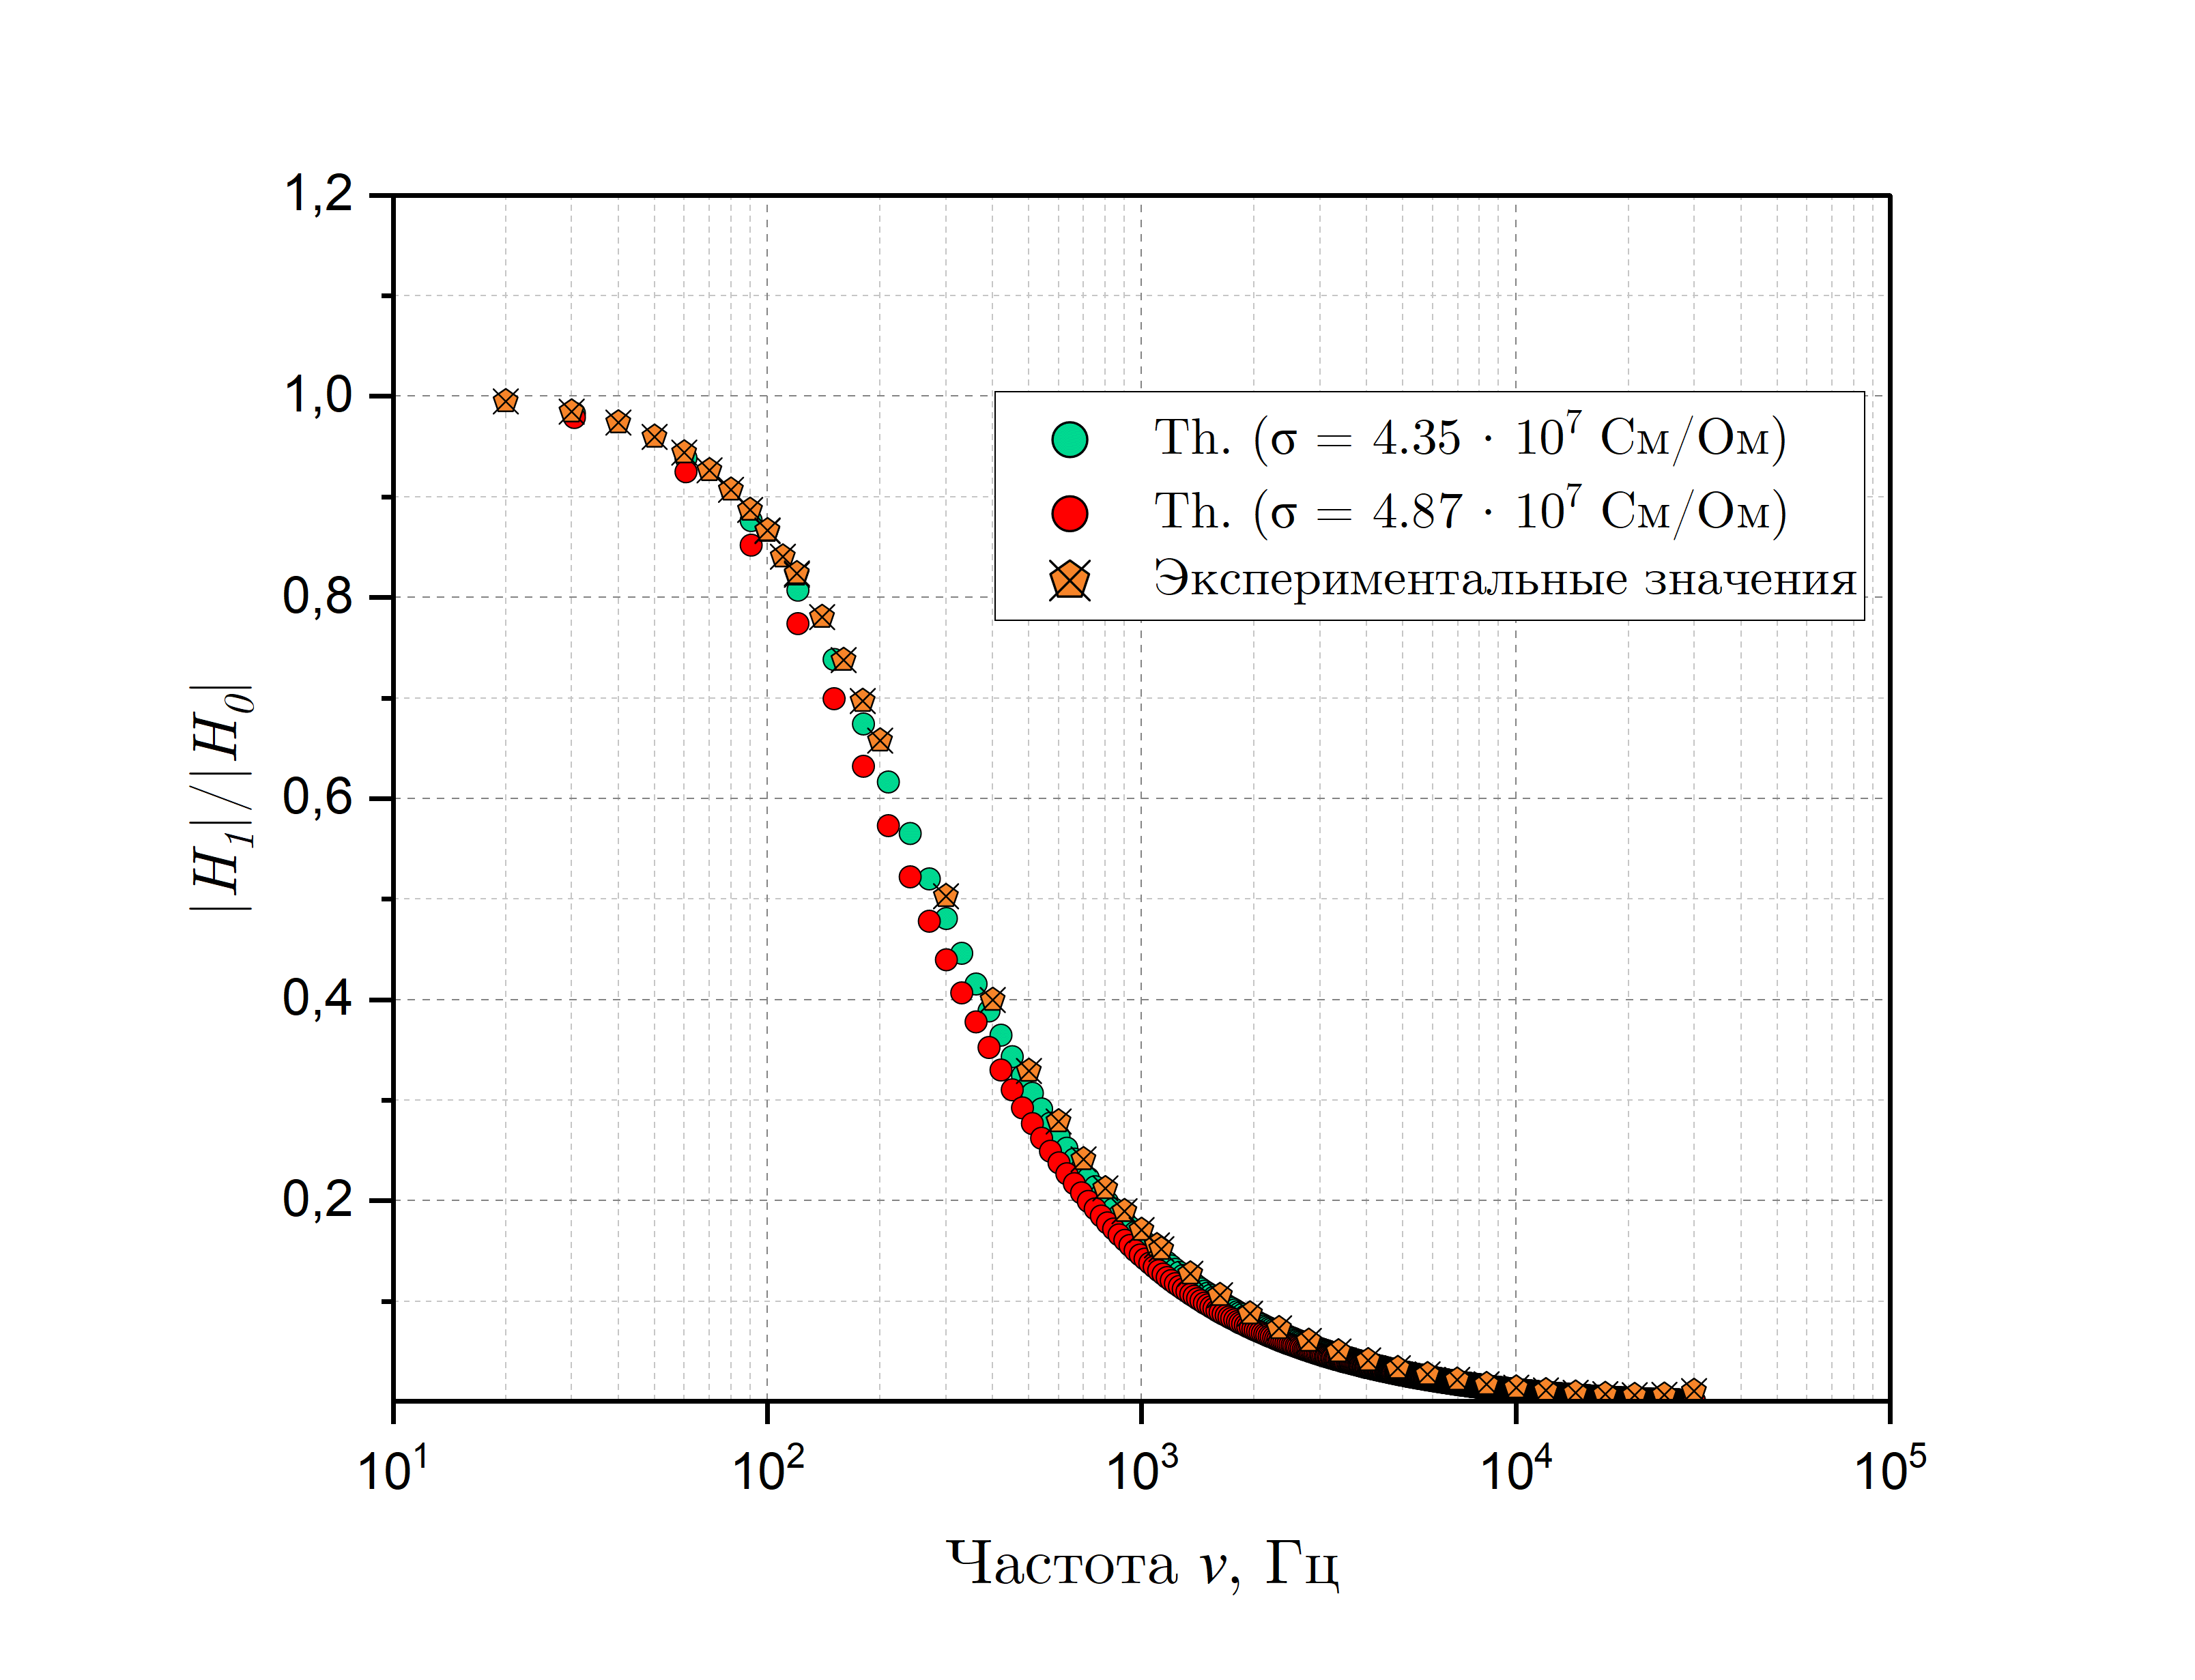
\includegraphics[width = 14 cm]{images/graph_ln_coeff.png}
        \caption{График зависимости $\lvert H_1 \rvert / \lvert H_0 \rvert$ от $\nu$}
        \label{graph:ln_coeff}
    \end{figure}

    \section{Заключение}

    Мы измерили проводимость материала цилиндра 4 разными способами. Итоговые значения приведены в таблице \ref{table:res}.

    \begin{table}[H]
        \centering
        \begin{tabular}{lccc}
        Метод измерения & $\sigma, 10^{7} См/м$ & $\Delta\sigma, 10^{7} См/м$ & $\varepsilon_{\sigma}$ \\
        \toprule
        Отношение амплитуд & 4,542 & 0,005 & 0,1\% \\
        Разности фаз (низкие частоты) & 4,470 & 0,070 & 1,5\% \\
        Разности фаз (высокие частоты) & 4,870 & 0,090 & 1,8\% \\
        Индуктивность & 4,350 & 0,020 & 0,5\%\\
        \end{tabular}
        \caption{Сравнение результатов различных методов}
        \label{table:res}
    \end{table}
    
    В установке в качестве экрана используется медная труба промышленного производства. Технология изготовления труб оказывает заметное влияние на электропроводимость. Из-за наличия примесей проводимость меди нашей трубы отличается от табличного значения (в меньшую сторону).

    Измерение проводимости с помощью исследования отношений амплитуд оказалось самым точным, самым неточным оказался метод измерения через разность фаз при высоких частотах. Погрешность измерения проводимости через разность фаз при низких частотах в основном связана с погрешностью измерения самой разности фаз, т.к. погрешность последней возрастает в несколько раз при подсчете тангенса угла.

\end{document}